\documentclass[10pt,a4paper]{book}

\usepackage{ardour,graphicx,afterpage,url,xstring,xcolor,titlepic,makeidx}
\makeindex

% XXX
% solo/mute model
% external sync
% connection management/routing
% snapshots
% undo/redo, how it doesn't work with, say, mixer settings
% control surfaces


% And may god bless the stackoverflow and all who sail in her
% http://tex.stackexchange.com/questions/5226/keyboard-font-for-latex
\usepackage[T1]{fontenc}
\usepackage[utf8]{inputenc}
\usepackage{tikz}
\usetikzlibrary{shadows}

\newcommand*\keystroke[1]{%
  \tikz[baseline=(key.base)]
    \node[%
      draw,
      fill=white,
      drop shadow={shadow xshift=0.25ex,shadow yshift=-0.25ex,fill=black,opacity=0.75},
      rectangle,
      rounded corners=2pt,
      inner sep=1pt,
      line width=0.5pt,
      font=\scriptsize\sffamily
    ](key) {#1\strut}
  ;
}

% XXX: format
\newcommand{\button}[1]{#1}
\newcommand{\menu}[1]{\emph{\StrSubstitute{#1}{,}{ $\rightarrow$ }}}
\newcommand{\key}[1]{\keystroke{\StrSubstitute{#1}{,}{ + }}}
\newcommand{\directory}[1]{\texttt{#1}}
\newcommand{\todo}[1]{\marginpar{\small\texttt{#1}}}
\newcommand{\modone}{Control}
\newcommand{\modtwo}{Alt}
\newcommand{\modtertiary}{Shift}

% Add a screenshot.
% Parameters are:
%   filename within screenshots/
%   caption
%   label
\newcommand{\screenshot}[3]{%
\begin{figure}[ht]%
\begin{center}
\includegraphics[scale=0.5]{screenshots/#1}
\end{center}
\caption{#2}
\label{#3}
\end{figure}}

\newcommand{\inlinetool}[1]{\includegraphics[scale=0.45]{screenshots/tool-#1.png}}

% Voodoo from http://answers.google.com/answers/threadview?id=282787
\definecolor{ListingGrey}{rgb}{0.8,0.8,0.8}
\makeatletter\newenvironment{listing}{%
   \medskip\begin{lrbox}{\@tempboxa}\begin{minipage}{\columnwidth}\ttfamily}{\normalfont\end{minipage}\end{lrbox}%
   \colorbox{ListingGrey}{\usebox{\@tempboxa}}\medskip%
}\makeatother

\title{Ardour 3 --- A users' manual}
\titlepic{
\includegraphics{graphics/ardour_bw.pdf}}
\author{Paul Davis\\Carl Hetherington}
\date{}
\begin{document}

\maketitle


\clearpage
\thispagestyle{empty}

\bigskip
\bigskip
\bigskip

\begin{quote}
\emph{``One of the secrets of life is that all that is really worth the doing is what we do for others''} --- Lewis Carroll (perhaps)
\end{quote}

\bigskip
\bigskip
\bigskip

\begin{quote}
\emph{``If you want to build a ship, don't drum up the men to gather wood, divide the work and give orders.  Instead, teach them to yearn for the vast and endless sea''} --- Antoine de Sant Exup\'ery (possibly)
\end{quote}

\bigskip

\tableofcontents


% ====================================================================================
% INTRODUCTION
% ====================================================================================

\chapter{Introduction}

Hello, and welcome to Ardour!

\section{What is Ardour?}

Ardour is an open-source digital audio workstation (DAW) for Linux and
Mac OS~X.

\section{Typographical conventions}

This manual uses special symbols to denote sections which contain
advanced material.  The reader can skip these sections without any
great loss.

\begin{danger}
Tricky parts of the text are marked with a `bend in the road' marker.
They contain extra information which may be of interest to advanced
users.
\end{danger}

\begin{ddanger}
Especially tricky parts of the text are marked with a double
bend-in-the-road marker.  Such sections will only be of interest to
the completist or serious hacker.
\end{ddanger}

When a menu option is discussed, it will look like this:

\menu{Menu option,Submenu option}




\section{About this manual}

This manual is a work-in-progress.  In other words, it is not even
close to being complete.  Any suggestions for improvements, content,
or comments on parts that do not make sense are welcome to
\url{cth@carlh.net}.

\begin{danger}
For those familiar with `git', the manual's \LaTeX\ source can be
obtained from the git repository linked from
\url{http://carlh.net/ardour}.  Patches to the manual are most welcome.
\end{danger}


\section{Getting help with Ardour}

There are several places that you can get help with using Ardour.

\subsection{The website}

Ardour's website (\url{http://ardour.org/}) contains many useful
resources, including a list of frequently-asked questions, a forum and
a bug and feature request tracker.

\subsection{IRC}
\index{IRC}

Ardour's core developers and several key users are usually to be found
on Internet Relay Chat (IRC) on \url{irc.freenode.net} in \#ardour and
\#ardour-osx at pretty much any hour of the day or night.  This is a
live chat system that is great for dicussing Ardour's development,
design, and also user problems.  There are IRC clients for most
operating systems, or you can join in directly from your web browser
by choosing \menu{Help,Chat} from within Ardour.

If you join the IRC rooms, here are a few tips:

\begin{itemize}
\item \emph{Don't ask to ask, just ask} --- rather than saying `Is it
  ok if I ask a question?', just ask your question --- it is not
  considered rude to do so.  Then wait: your answer may come in
  seconds, minutes, hours or never, depending on who is around and
  what time of the day it is wherever they happen to be in the world.
  In particular, make sure you \emph{do} wait; do not get upset if you
  don't get an answer straight away.
\item \emph{Don't be offended if no-one replies} --- although other
  users may be logged into the channel, they may well be coding
  Ardour, cooking, reading XKCD, cleaning their ostrabagalous devices,
  or any number of other things.
\item \emph{Don't paste large amounts of text into the channel} --- if
  you have more than a couple of lines of output from some command
  that you want to show everyone, use a site like \url{pastebin.com}.
  You can copy your text into that site, and it will give you a web
  address that you can paste into the channel.
\item \emph{Be as detailed as possible} --- if you have a problem,
  tell us what version of Ardour you are using, and what operating
  system you are running on (Linux, OS X or Windows).
\end{itemize}


\subsection{Mailing lists}

There is a Ardour users mailing list, where various discussions about
Ardour (and recording in general) take place.  There are links to join
the list on Ardour's website.


\subsection{Support expectations}

As Ardour evolves, it becomes a serious alternative to commercial
products for more and more people. We see the download counts increase
for each new release, and the volume of traffic on the mailing lists
is growing. That's lovely, of course. We work on Ardour without the
accoutrements of a `normal' software corporation, so whenever a new
user finds our work useful and worthwile, it makes what we do seem
meaningful and worth continuing with.

Unfortunately, it's not all roses we receive.  With wider public
interest and more users, there's bound to be people who are
disappointed in Ardour. We believe, however, that it's only because
most newcomers do not realize what to expect.


\subsubsection{The development team}

Many users probably don't realize it, but the development team driving
Ardour forward is very small for the amazingly complex piece of
software that is a contemporary DAW\@.

At this time, the main force behind Ardour is delivered by one person,
with core aid from two others, and contributions from on the order of
a dozen others. Consider that we do support, web site maintenance,
documentation, feature enhancements, debugging, as well as
development.

There are more people (perhaps another dozen) pitching in with
translation, release engineering (preparing Ardour for users), Mantis
triaging (`Mantis' is the bug database used to keep track of known
problems, `triaging' the process of prioritizing and verifying bugs)
and other necessary tasks.

So we are always looking for new people to help, and while
(unfortunately) a common misconception is that a project like Ardour
would only benefit from more programmers, it is not the case! Whatever
your ability, we can use it. If you are interested in spending a
little time making Ardour a better DAW, please don't hesitate to join
the developer mailing list and offer your services.

\subsubsection{Ardour features and polish}

As Ardour is getting more powerful and usable, we attract more and
more users who expect the same feature set and product polish as
they'll find in a commercial product such as DigiDesign's ProTools or
Steinberg's Nuendo. This isn't the right way to think about Ardour at
this time.

Not that we don't want to get there, you understand, but it's simply
not a reasonable comparison. DigiDesign has spent who knows how many
man-hours worth of development on ProTools and can spend a lot on
getting good documentation written, new features, debugging,
installation process made smooth and generally polish the thing till
it shines. In comparison, Ardour development is driven primarily by
the interests of just a few people. Development is a full time job for
the lead developer, who also raises a three kids, fixes up his house,
has friends and even a relationship with a gorgeous woman.

Do not read that as an excuse for why Ardour lacks in comparison with
other products. Do read it as an explanation for why you should expect
nothing more from Ardour than it actually delivers. And rest assured
that the developers want and expect it to rival, or better yet, beat
the proprietary DAWs. That's why we're so committed to this
development model --- because we believe it's the best way to get there.

\subsubsection{Releases}

Ardour releases are also put together by volunteers. This means that
there's usually only prebuilt binaries available for a few select
platforms. While we would like to see Ardour prebuilt for all the
platforms (and operating system versions) Ardour runs on, it's simply
not possible since the volunteers doing the release only have access
to a subset of those platforms.

With specific regards to library dependencies: depending on the
volunteer's machine configuration, the Ardour binary may require you
to install additional or newer libraries before it will work. If so,
the installation instructions should contain the necessary information
for you to find those libraries. Please do not complain about the need
for these libraries --- just as you might dislike installing/upgrading
the libraries, the volunteer doing the release may dislike
removing/downgrading the libraries on her machine.

If you find that there are no prebuilt binaries for your
platform/configuration, and are willing to help provide packages for
coming releases, please join the developer mailing list and offer your
services. It is not a requirement that you are a programmer, but there
may be a requirement for (commercial) development tools which not
everyone would have access to. If you have the time and tools, we can
probably guide you through the process, even if you don't have the
knowledge.

\subsubsection{Support}

You can join both the user and developer mailing lists and ask
questions there. You can also ask for help on IRC, and you can file
bug reports and feature requests in Mantis. However, since support is
also provided on a volunteer basis, you must be careful not to have
unreasonable expectations: you cannot demand your questions to be
answered or bugs to be fixed. In short: the people volunteering time
to Ardour only have so much time available, and they alone decide how
to spend it. Please respect their choice.

When that is said, you should know that the mailing list and the IRC
channel are friendly places --- few requests go without reply. And we
also do our best to fix all bugs reported, just as we strive to
implement requested features. But as should be evident from the number
of open bugs in Mantis, there's not enough hours in the day to allow
us to address all issues in a timely manner.





% ====================================================================================
% OVERVIEW
% ====================================================================================

\chapter{Overview}

As one might expect, Ardour is similar in many ways to many other DAWs
and also has its fair share of differences.  This chapter gives an
overview of Ardour.


\section{JACK}
\index{JACK}

Ardour is built on another piece of software called JACK\footnote{JACK
  stands for the JACK Audio Connection Kit; a pleasingly recursive acronym}.
JACK has two main functions; first, it moves audio and MIDI to
and from a sound card, and second, it allows audio and MIDI to be
routed between different applications.

JACK provides a great deal of flexibility and power, especially when
running other applications (such as soft-synthesizers or samplers) at
the same time as Ardour.  It is somewhat similar to Steinberg's Rewire
technology, though broader in scope.  It is even possible to use JACK
to route audio and MIDI over network connections.

JACK is so important to Ardour's operation that it earns its own
discussion in Chapter~\ref{ch:jack}.


\section{Ardour concepts}

Ardour has its own names for the usual set of common DAW concepts.
This section briefly describes some of these concepts.


\subsection{Sessions}
\index{session}

An Ardour \emph{session} is a container for an entire project.  A
session may contain an arbitrary number of tracks and busses
consisting of audio and MIDI data, along with information on processing
those tracks, a mix of levels, and everything else related to the
project.  A session might typically contain a song, or perhaps an entire
album or a complete live recording.

Ardour sessions are held in directories; these directories contain one
or more \emph{session files}, some or all of the audio and MIDI data
and a number of other state files that Ardour requires.  The session
file describes the structure of the session, and holds automation data
and other details.

\begin{danger}
Ardour's session file is kept in XML format, which is advantageous as
it is somewhat human-readable, and human-editable in a crisis.  Sound
files are stored in one of a number of optional formats, and MIDI
files as SMF (standard MIDI format).

It is also possible for Ardour sessions to reference sound and MIDI
files outside the session directory.
\end{danger}

Ardour has a single current session at all times; if Ardour is started
without specifying one, it will offer to load or create one.



\subsection{Tracks}
\index{track}

A track is a concept common to most DAWs, and used also in Ardour.
Tracks can record audio or MIDI data to disk, and then replay it with
processing.  They also allow the audio or MIDI data to be edited in a
variety of different ways.

In a typical pop production, one might use a track each for the kick
drum, another for the snare, more perhaps for the drum overheads and
others for bass, guitars and vocals.

Ardour can record to any number of tracks at one time, and then play
those tracks back.  On playback, a track's recordings may be processed
by any number of plugins, panned, and its level altered to achieve a
suitable mix.

\begin{danger}
A track's type is really only related to the type of data that it
stores on disk.  It is possible, for example, to have a MIDI track
with a synthesizer plugin which converts MIDI to audio.  Even though
the track remains `MIDI', in the sense that its on-disk recordings are
MIDI, its output may be audio-only.
\end{danger}


\subsection{Regions}
\index{region}

A track may contain many segments of audio or MIDI\@.  Ardour contains
these segments in things called \emph{regions}, which are
self-contained snippets of audio or MIDI data.  Any recording pass,
for example, generates a region on each track that is enabled for
recording.  Regions can be subjected to many editing operations; they
may be moved around, split, trimmed, copied, and so on.


\subsection{Playlists}
\index{playlist}

The details of what exactly each track should play back is described
by a \emph{playlist}.  A playlist is simply a list of regions; each
track always has an active playlist, and can have other playlists
which can be switched in and out as required.


\subsection{Busses}
\index{bus}

Busses are another common concept in both DAWs and hardware mixers.
They are similar in many ways to tracks; they process audio or MIDI,
and can run processing plugins.  The only difference is that their
input is obtained from other tracks or busses, rather than from disk.

One might typically use a buss to collect together the outputs of
related tracks.  Consider, for example, a 3-track recording of a
drum-kit; given kick, snare and overhead tracks, it may be helpful to
connect the output of each to a bus called `drums', so that the
drum-kit's level can be set as a unit, and processing (such as
equalisation or compression) can be applied to the mix of all tracks.


\subsection{Plugins}
\index{plugin}

Ardour allows you to process audio and MIDI using any number of
\emph{plugins}.  These are external pieces of code, commonly seen as
VST plugins on Windows or AU plugins on Mac OS~X.  Generally speaking,
a plugin is written using one (and maybe more) standards.  Ardour's
plugin support is for the following standards:

\begin{itemize}
\item LADSPA\footnote{An acronym of ``Linux Audio Developers' Simple
  Plugin API''} --- the first major plugin standard for Linux.  Many
  LADSPA plugins are availble, mostly free and open-source. \index{LADSPA}
\item LV2 --- the successor to LADSPA.  Lots of plugins have been
  `ported' from LADSPA to LV2, and also many new plugins written. \index{LV2}
\item VST --- Ardour supports VST plugins that have been compiled for Linux. \index{VST}
\item AU --- Mac OS~X versions of Ardour support AudioUnit (AU) plugins. \index{AU}
\end{itemize}

Ardour has some support for running Windows~VST plugins on Linux, but
this is rather complicated, extremely difficult for the Ardour
developers to debug, and generally unreliable.  If it is at all
possible, you are strongly advised to use native LADSPA, LV2 or Linux
VST plugins on Linux, or AU on Mac OS~X\@.


\section{The Ardour interface}

This section gives an overview of Ardour's main interface elements.

\subsection{The editor window}
\index{editor}

The first of Ardour's two main windows is the \emph{Editor}.  A
typical editor window is shown in Figure~\ref{fig:typical-editor}.

\begin{figure}[ht]
\begin{center}
\includegraphics[scale=0.75]{diagrams/editor-summary.pdf}
\end{center}
\caption{A typical editor window}
\label{fig:typical-editor}
\end{figure}

The main bulk of the window is taken up with the timeline; this is the
area in which regions and automation are displayed, with time moving
from left to right.  The track controls area gives a set of controls
for each track, for basic operations such as solo, mute and so on.
The (optional) editor mixer is a single mixer strip which handles the
currently-selected track, and is useful for tweaks to the mix without
the need to move to the full mixer window.  At the bottom of the
window is the `summary', which displays the whole session in a
reduced-size form.  At the top right is a bar of useful information
about the state of the system.

The operation of the editor window is described in more detail in
Chapter~{\ref{ch:editor-window}.

\subsection{The mixer window}
\index{mixer}





% ====================================================================================
% JACK
% ====================================================================================

\chapter{JACK}
\label{ch:jack}
\index{JACK}

\section{Introduction}

JACK is the JACK audio connection kit.  It is a piece of software that
provides the low-level `plumbing' which allows Ardour to work.  Its
setup is crucial to Ardour; Ardour will not work without it.

JACK's essential task is to route audio and MIDI data to and from a
sound card, and also between applications.  It manages a set of
\emph{ports}, which it can connect together in arbitrary ways.
Figure~\ref{fig:typical-jack-session} gives a diagram of a moderately
complex JACK session.

\url{jackaudio.org/pulseaudio_and_jack}

\begin{danger}
JACK is not limited to the standard concept of the `sound card'.  You
may choose to have no sound card at all (in which case JACK can run in
`dummy' mode).  It is also possible to send signals to and from JACK
over TCP/IP networks using netjack.  For simplicity, this manual will
assume that the user has a sound card in the conventional sense.
\end{danger}

\subsection{JACK and other audio software}

JACK is designed so that it uses a single sound-card, and has
exclusive control of that sound-card while it is running.  This is a
couple of consequences.  Firstly, if the sound card used to capture
audio is different from the one used to play it back, complications
arise.  Secondly, other software which tries to obtain exclusive
control of your sound-card, most notably `pulseaudio', may interfere
with JACK's operation.

\subsubsection{JACK with multiple sound cards}
\label{sec:jack-multiple-cards}

If at all possible, it is a good idea to use JACK with a single sound
card.  Correctly using more than one card at the same time is
difficult.  The main reason for this difficulty is that JACK assumes
that all sound cards and programs that it is connecting are running
with synchronised sample clocks.  Arranging this is not easy if there
are two cards; there will be two unsynchronised sample clocks.

If you accept that using multiple sound cards is going to be
difficult, and you want to do it anyway, there are a number of
approaches.  These are described in Appendix~\ref{ap:advanced-jack}.

\subsection{Will my sound card work?}

For your sound card to work with JACK, must have a driver suitable for
the operating system that you are running on.  For Linux, this means
that your card must be supported by ALSA or FFADO; ALSA supports
drivers using a wide variety of interfaces, and FFADO is for firewire
soundcards only. 

The easiest way to check on ALSA compatibility is to visit
\url{http://www.alsa-project.org/main/index.php/Matrix:Main}.  This is
the ALSA soundcard matrix and describes ALSA's support for a variety
of cards.  For FFADO, consult
\url{http://www.ffado.org/?q=devicesupport/list}.

For Mac OS~X, any card that is supported by the operating system
should work fine.


\subsection{JACK versions}

For historical reasons, there are two `branches' of JACK that are both
maintained, and can be used as drop-in replacements for each other.
JACK1 has version numbers like 0.121.3, and JACK2 (also known as
jackdmp) has version numbers like 1.9.8.  Both implementations have
their advantages and disadvantages.  It does not matter a great deal
which one you use.

% XXX: unless what?


\section{Starting JACK}

Ardour can start JACK automatically when it starts; and indeed many
users will find that this works perfectly well.  It is also possible
to start JACK manually, either at the command line or using a tool
such as QJackCtl\footnote{\url{http://qjackctl.sourceforge.net}} (on
Linux) or JackPilot\footnote{\url{http://www.jackosx.com}} (on Mac
OS~X).

\subsection{Parameters}

JACK has many parameters which affect its operation.  Some of the more
important ones are discussed here.

\subsubsection{Sampling rate}

This is the number of samples per second that JACK will process, and
is important as it will govern the sampling rate that all audio
applications will run at.  The chosen rate must be supported
by the sound card, so values such as 44.1kHz, 48kHz, 96kHz
et.\ cetera are typical choices.  The higher the sampling rate, the
higher the theoretical audio frequency that the system can reproduce,
but also the more disk space will be consumed by audio recordings, and
the more CPU power will be required to run audio plugins.

The arguments about the best sampling rate are many, long and varied,
but can (in the humble opinion of the author) be summarised as: `if in
doubt, use 44.1kHz, as no-one can hear the difference between that and
anything higher (though they may think they can)'.

\subsubsection{Frames per period}

In a move necessary for efficiency, JACK does not process audio
sample-by-sample, but in blocks of samples.  The size of these blocks
can be selected when starting JACK\@.  A block is called a `period',
and samples are often known as `frames' in the context of JACK\@.  If
the frames per period count is made smaller, the latency experienced
by sounds going into and coming out of the computer will be reduced;
on the other hand, smaller buffers make the computer work harder, and
may result in other problems if the computer is not well set-up.  It
is usually difficult to get below 64 frames per period on a typical
desktop computer, and values as high as 2048 frames per buffer are
perfectly acceptable if you do not particularly care about latency.

\begin{danger}
The frames per period value governs how often JACK will talk to the
sound card.  If, for example, JACK is set to 64 frames per period, the
sound card will tell JACK when it has 64 new frames ready; JACK (and
therefore Ardour) must then respond before the next 64 frames arrives.
This has the consequences that JACK and Ardour are awoken more often,
causing a greater CPU load, and that the requirements for JACK's
response time are much more critical with smaller period sizes.  Some
systems will struggle to wake JACK up in time, making larger period
sizes more reliable on those systems.
\end{danger}

\subsubsection{Number of periods}

This value is related to the frames-per-period value above; 2 is
typical, and will work for most sound cards and systems.  It is worth
trying 3 here if problems are experienced.


\section{Troubleshooting JACK}

\subsection{I am getting lots of xruns!}
\label{sec:xruns}

An \emph{xrun} \index{xrun} is JACK's way of saying that the sound
card wanted attention, but JACK could not provide it quickly enough.
The causes of xruns are many and various.  The remainder of this
section lists some common causes of xruns.


\subsubsection{Buffer size or period count too small}

The JACK `buffer size', or number of frames per period, governs how
often JACK has to talk to the sound card; smaller buffer sizes require
JACK to communicate with the sound card more often and with tighter
deadlines.  Increasing buffer size can be a simple way to reduce
xruns.

Similarly, if you have a lot of xruns, particularly with a USB device,
try increasing JACK's period count from 2 to 3.


\subsubsection{JACK not running with real-time privileges}

JACK will try, by default, to obtain \emph{real-time} scheduling
privileges when it starts.  If it suceeds, it means that the
operating system will treat JACK as higher priority than some other
tasks when it needs to talk to the soundcard, which is very likely to
reduce the incidence of xruns.

Some versions of Linux are careful about which tasks are allowed
real-time priviledges, as there is potential for such tasks to cause
problems with the system.  As a result, JACK may fail to obtain
real-time privileges, in which case your Linux configuration must be
altered to allow JACK to get what it wants.  For Debian- and
Ubuntu-based distributions, the best way is usually to add your user
to the `audio' group using

\begin{listing}
usermod -a -G audio fred
\end{listing}

where \texttt{fred} is your user ID\@.  After this, configure the audio
group to be allowed appropriate settings by editing
\texttt{/etc/security/limits.conf} and adding

\begin{listing}
@audio - rtprio 99\\
@audio - memlock unlimited
\end{listing}

to the bottom of of the file.  This allows members of the audio group
to start tasks with high real-time (RT) priority, and also allows them
to lock their memory into `real' memory; this is another step that
improves real-time performance.

After making these changes you will need to log out and log back in
again to see the effects.

\todo{Denormals?}
\todo{CPU frequency scaling?}

\subsection{I can play back but I cannot record, or vice versa}

This is commonly caused by JACK's prediliction for using only
one sound card.  If you are using different sound cards for playback
and record (which will be the case even if you are doing playback via
HDMI and recording via an on-board sound-card) you will need to set
JACK up to use multiple sound cards, as discussed in
Appendix~\ref{ap:advanced-jack}.



% ====================================================================================
% QUICK START
% ====================================================================================

\chapter{Quick start}
% XXX: links to things later on

This chapter blithely assumes that you just want to use Ardour to make
a basic audio recording from a sound card, and describes how that can
be achieved.  We assume that you have some sound source (such as a
microphone, guitar or whatever) plugged into one of your sound card's
inputs, and a monitoring system (speakers or headphones) connected to
its outputs.


\section{Starting Ardour and creating a session}

When Ardour is run for the first time, it starts with the dialogue box
shown in Figure~\ref{fig:welcome-to-ardour}.  Click \button{Forward} to continue.

\screenshot{welcome-to-ardour.png}{Welcome to Ardour!}{fig:welcome-to-ardour}

As it is the first run, Ardour now asks a few basic questions about
how it should be set up.  Its first question is about where to put
sessions by default, as shown in
Figure~\ref{fig:default-folder-for-new-sessions}.  The initial choice
will be the your home directory; other locations can be selected by
clicking on the button and selecting an alternative directory.

\screenshot{default-folder-for-new-sessions.png}{Default folder for new sessions}{fig:default-folder-for-new-sessions}

The next choice governs how Ardour will handle monitoring, as shown in
Figure~\ref{fig:monitoring-choices}.  For the purposes of this test,
choose `Ask Ardour to playback material as it is being recorded', as
this makes things slightly clearer in many cases.

\screenshot{monitoring-choices.png}{Monitoring choices}{fig:monitoring-choices}

Following this, Ardour asks for a choice with respect to a monitor
section (see Figure~\ref{fig:monitor-section}).  This is explained in
more detail later; for now, just choose the default `use a master bus
directly'.

\screenshot{monitor-section.png}{Monitor section}{fig:monitor-section}

At this point, if JACK has not already been started, Ardour will try
to do it for you.  In order to do that, it asks about how JACK should
be set up (Figure~\ref{fig:audio-midi-setup-device}).

There are three pages to the Audio / MIDI setup dialogue; the first is
`device', which allows selection of the sound card that Ardour will
use, the sampling rate at which it will operate, and the buffer size.
For now, select the interface that you are using for recording and
leave other options as they are.  For more information on the options
here, consult Chapter~\ref{ch:jack}.

\screenshot{audio-midi-setup-device.png}{Audio/MIDI setup --- device}{fig:audio-midi-setup-device}

The final step in creating our session is to give it a name, as in
Figure~\ref{fig:new-session}.  Enter something like `test' and click
\button{Open}.  At last, the reward should be the editor window
(Figure~\ref{fig:editor}).  The session is created!

\screenshot{new-session.png}{New session}{fig:new-session}

\begin{figure}[ht]
\begin{center}
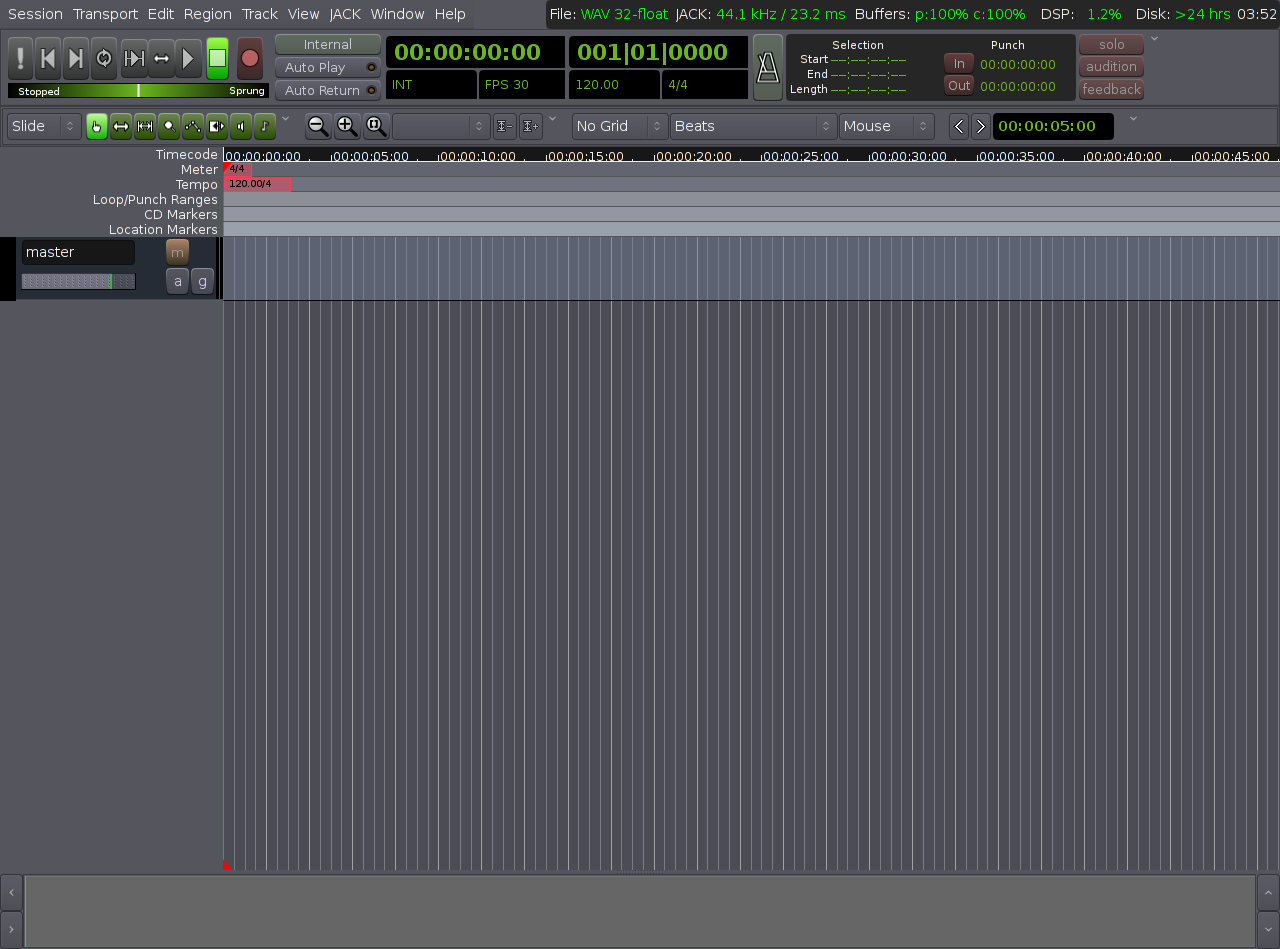
\includegraphics[scale=0.3]{screenshots/editor.png}
\end{center}
\caption{\ldots and finally: the editor!}
\label{fig:editor}
\end{figure}

\section{Adding a track and connecting it up}

The next step is to add a track to our session so that we have
something to record onto.  Choose \menu{Track,Add Track or Bus...}
from the menu at the top of the editor window.  This will bring up a
dialogue box, as shown in Figure~\ref{fig:quickstart-add-track-or-bus}.

\screenshot{add-track-or-bus.png}{`Add Track or Bus' dialogue}{fig:quickstart-add-track-or-bus}

For now, leave the options as they are; this will create a single
monophonic audio track.  This track must now be connected to the sound
card so that it can record incoming audio.

Perhaps the easiest way to connect up this new track is to open its
editor mixer strip.  Do this now by pressing \key{Shift,E} or
choosing \menu{View,Show Editor Mixer} from the main menu.  The top of
the mixer strip that appears looks like that in
Figure~\ref{fig:top-of-mixer-strip}.

\screenshot{top-of-mixer-strip.png}{Top part of a mixer strip}{fig:top-of-mixer-strip}

At the top of this mixer strip there are three main buttons.  The
first, labelled `Audio 1' (the name of the track) can be clicked on to
open a menu of options for the track.  The second, marked `1' is the
input selector, and the third, marked $\phi$, is a button to invert
the track's signal.

In order to look at the connections to the input of this track,
left-click on the button marked `1' to open the input \emph{port
  matrix}, as shown in Figure~\ref{fig:input-port-matrix}.

\screenshot{input-port-matrix.png}{Input port matrix}{fig:input-port-matrix}

The port matrix is the main interface that Ardour offers for
connecting things together.  In our example matrix, the left-hand side
shows a set of ports that generate audio data; these correspond to the
sound card inputs, outputs of Ardour busses and tracks, and other
things that may exist on the system.  Different groups of these ports
can be seen by choosing one of the tabs on the far left-hand side of
the dialogue.

At the bottom of the dialogue is the input to our track.

In the example matrix, there is a green dot at the intersection of the
`L' part of `in $1+2$' and the `Audio 1 in' port.  This means that the
input of the `Audio 1' track hardware input 1.  Change this
connection, if necessary, by clicking on the square which corresponds
to the input to record from.  At this point, the Audio 1 meter should
display any signal that is being sent into the sound card.  If this is
not working, something has gone wrong.

\section{Recording}

At this point, Ardour is receiving a signal from some external sound
source via the sound card.  It is now possible to make a test
recording.  Click the record-enable buttons (red buttons with a pink
circle) in both the `Audio 1' track controls and the main transport
controls (shown in Figures~\ref{fig:track-controls} and
\ref{fig:transport-controls} respectively, then click `Play' to start
the transport.

\screenshot{track-controls.png}{Track controls area}{fig:track-controls}
\screenshot{transport-controls.png}{Main transport controls}{fig:transport-controls}

Ardour is now recording; the play-head will move, and a red rectangle
will be drawn where the recording is taking place.  Make a noise with
your external sound source!  When you have finished recording, click
the Stop button in the transport controls area.  You should now have a
region containing your recording on the `Audio 1' track, as in
Figure~\ref{fig:recorded-one-region}.

% \screenshot{recorded-one-region.png}{Editor window after recording a region}{fig:recorded-one-region}

\section{Playing back your recording}

Now we can play back the audio that you have just recorded.  First,
you will need to move the playhead back to a point before your
recorded region.  Perhaps the easiest way to do this is to click
somewhere within the rulers area of the editor window.

% some picture of where this is, or a back-link to the editor window

Once the playhead is located before your recording, click the `Play'
button (or press the spacebar on the keyboard) to start playback.  You
should hear your recording through your monitor speakers or
headphones.

\section{Adding another track as an overdub}

Now we can experiment further by adding an overdub to the first
recording.  First, add a new track, as we did before, and connect it
up to the input on your soundcard which your source is connected to.

Now, record-enable the new track, move the playhead to before the
previously recorded region, make sure the session is record-enabled
and start the transport (by clicking `Play' or pressing the spacebar).
You should hear the previously-recorded audio on your monitor system
while the new recording is in progress.  Record something suitable
over the top of your first region.

We now have two tracks of recorded data; you might like to add some
more!

\section{Mix-down}

We will now assume that you want to do a mix-down of your magnum opus
into a stereo WAV file.  Such a file could later be converted to an
MP3, or burned to CD, or simply played-back as-is by some other media
player on your computer.  

First, we need to mix the tracks that you have recorded so that they
sound as you want them to.  We will cover much more advanced mixing
and processing later, but for now we will just set the relative levels
of the two tracks.  The easiest way to do this is to open the
\emph{mixer} window, either by selecting \menu{Window,Mixer} or by
pressing \key{Alt,M}.  The mixer window is shown in Figure~\ref{fig:mixer-window}.

% \screenshot{mixer-window.png}{The mixer window}{fig:mixer-window}

Here you will see a mixer strip for each track that you have recorded,
and a `master' strip.  The signals for each track flow from the
recordings on disk, through the appropriate strip, and they are then
mixed together and passed through the master strip.  The bottom half
of each mixer strip contains a \emph{fader}; this controls the level
of each track.  You can adjust the levels of each of your recordings
by dragging the mixer strip; the green marker indicates 0dBFS (`unity
gain'), at which the level of the track will be unaltered from the
recording.

Play back your recordings from the editor window, and experiment with
the levels in the mixer window until you have a sound that you are
happy with.


\section{Export}

The final step is to export our recording into a stereo WAV file.
Ardour's export options are extensive, but for now we will keep it
simple.  Choose \menu{Session,Export,Export to Audio Files} from the
editor menu, and the \emph{Export} dialogue will open, as shown in
Figure~\ref{fig:export-dialogue}.

First, we have to specify the format that we will export in.  Fill in
the \emph{Label} field with some name like `WAV for CD', then click
the \button{New} button beside the Format entry in the dialogue, and
click on \button{CD}, \button{Lossless (linear PCM)}, \button{WAV} and
\button{44.1kHz} entries.  Then click \button{Save} to save the export
preset.  Enter some label for the export in the \emph{Location}
section, then click \button{Export}.  Ardour will mix your session
down to a WAV file and save it in the \directory{export} subdirectory of
your session folder.


% ====================================================================================
% THE EDITOR WINDOW
% ====================================================================================

\chapter{The editor window}
\label{ch:editor-window}
\index{editor}

A typical Ardour editor window is shown in Figure~\ref{fig:typical-editor2}.

\begin{figure}[ht]
\begin{center}
\includegraphics[scale=0.75]{diagrams/editor-summary.pdf}
\end{center}
\caption{A typical editor window}
\label{fig:typical-editor2}
\end{figure}

This window is where audio and MIDI material can be viewed, edited and
manipulated.  It offers a view of your session as it progresses in
time, and allows the constituent parts (tracks, regions, playlists and
so on) to be manipulated.  The contents of the main body of the window
represent the session's tracks and busses, the functionality of which
is discussed in Chapter~\ref{ch:tracks-and-busses}.

The remainder of this chapter discusses the other parts of the editor window.


\section{The playhead}
\index{playhead}

The red vertical line with arrow heads at either end is the called the
`playhead'.  The playhead position is used in a few different ways,
but the most obvious is that it lies at the point in time at which
Ardour is currently playing back or recording (or would be, were play
or record to be started).  It is also used in some editing operations,
as we will discuss later.


\section{The toolbar}
\index{toolbar}

The toolbar is a set of buttons that change the way the mouse and
keyboard interact with the regions on the tracks, in order to perform
different tasks.

Figure~\ref{fig:toolbar-annotated} shows the buttons on the toolbar.

\begin{figure}[ht]
\begin{center}
\includegraphics{diagrams/toolbar-annotated.pdf}
\end{center}
\caption{The Ardour toolbar}
\label{fig:toolbar-annotated}
\end{figure}

We will examine the broad function of these tools here, and go into
more detail on their operation later.

\begin{itemize}
\item \textbf{Select/move objects} (\key{o}) --- used to mark
  regions or MIDI notes as `selected', and to move them around (in
  time, or to a different track, or to a different note in the case of
  MIDI).
\item \textbf{Smart mode} --- this provides a combination of the
  functionality of `select/move objects' and `select/move ranges'
  which may be familiar to users of Pro~Tools.
\item \textbf{Select/move ranges} (\key{r}) --- used to mark
  ranges of time and to manipulate them.
\item \textbf{Zoom range} (\key{z}) --- this provides a mode whereby a time
  range can be dragged with the mouse, and the editor window will zoom
  to show that time range.
\item \textbf{Region gain} (\key{g}) --- used to edit audio
  gain curves on regions.
\item \textbf{Stretch/shrink} (shortcut key `t') --- allows stretching
  or shrinking of regions in time (using time-stretching /
  pitch-shifting algorithms) or MIDI notes.
\item \textbf{Listen} -- \todo{}
\item \textbf{Draw/edit MIDI notes} --- used to draw new MIDI notes
  into MIDI regions, or change the length of those that are already
  there.
\item \textbf{Edit region contents} (\key{e}) --- this is a
  kind of `modifier' for the other tools.  When selected, it means
  that the other tools will operate on region contents rather
  than the regions themselves.  For example, the select/move tool will
  select and move MIDI notes rather than the regions that the notes
  are in.
\end{itemize}

\section{Rulers}

The rulers section of the editor gives the option of several views;
some time indications, in different units, details of tempo and meter
(time signature) changes, and a display of various types of marker.

Right-clicking over the marker area offers a menu from which the
displayed rulers can be chosen.

\subsection{Time displays}

The time rulers that can be displayed are:
\begin{itemize}
\item \textbf{Min:Sec} --- time in hours:minutes:seconds:millseconds.
\item \textbf{Timecode} --- time in hours:minutes:seconds:frames.
\item \textbf{Samples} --- time in audio samples.
\item \textbf{Bars:Beats} --- time in bars and beats.
\end{itemize}

\subsection{Meter and tempo}

Ardour provides support for considering a piece of music as having
tempo and meter.  This is optional in the sense that you can happily
ignore tempo and meter settings if they are not relevant to your
recording situation.

Use of tempo has two main effects; firstly, Ardour can provide a
metronome `click' which can be used as reference to record to.
Secondly, tempo will affect the speed at which MIDI data is played
back, so you can change how your records will sound by changing the
tempo.

Meter (time signature) also affects the metronome click, as the click
will emphasise the sound of the first beat of the bar.  It has no
effect on the \emph{playback} of MIDI, but adjusting time signature to
match the music may make things more intuitive to work with.

Both tempo and meter affect the grid that is displayed (and,
optionally, snapped to) which shows bars and beats.  The grid will
adjust itself to zoom level, so the finer details of the session may
not be visible if you are zoomed too far out.

\subsection{Markers}

Ardour supports a variety of markers for various purposes.  Markers
can either be a single point in time or a range of time.

The basic marker types for general purpose use are \emph{location
  markers} and \emph{range markers}.  Location markers are a point in
time, and range markers represent, as one might expect, a time range.  

There are some other special marker types.  CD markers are intended to
indicate track marks for CD productions.  If a session has CD markers
at the start of each track, Ardour can generate a table-of-contents
for use with audio exports to allow them to be burnt to CD correctly.

Two special range markers are the `loop' and `punch' ranges.  The loop
range can be played back in a loop when the \emph{play loop range}
button is clicked.  The punch range will be used with punch-in
recording.


\section{Clocks}

This area contains two clocks, the primary and secondary.  They both
show the location of the playhead, but can be set to different time
representations.  By default, for example, the primary clock shows
position as a time-code, and the secondary shows bars, beats and
ticks.

Right-clicking on a clock pops up a menu from which you can choose the
time representation from one of the following:

\begin{itemize}
\item \textbf{Timecode} --- shows time as
  hours:minutes:seconds:frames.  The number of frames per second is
  set by the session property `timecode frames-per-second' (see
  Section~\ref{sec:session-properties-timecode}).
\item \textbf{Bars:Beats} --- shows time as
  bars\textbar{}beats\textbar{}ticks (there are 1920 ticks per beat).
\item \textbf{Minutes:Seconds} --- shows time as
  hours:minutes:seconds:milliseconds.
\item \textbf{Samples} --- shows time as samples (according to the
  sampling rate that JACK is using).
\end{itemize}

In addition to the time, the clock shows some other information.

When set to `timecode', the clock also shows the timecode reference
source; this defaults to `INT' for internal, but can also be `JACK' if
JACK is the timecode reference, `MTC' if Ardour is syncing to MIDI
time-code or `M-Clock' if Ardour is synced to MIDI clock.  To the
right of the timecode reference is the number of frames per second
(suffixed by `D') if drop-frame is being used.

In `Bars:Beats' mode, the area underneath the time shows the tempo (in
beats per minute) and time signature that are currently in effect.

\section{Times area}

The times area of the editor window shows a few useful bits of
information about any current selection and punch in/out range.  The
`selection' area shows the start, end and length of anything that is
currently selected (which may be a set of regions, a time range, or
whatever).  The `punch' area shows the punch range, and also whether
punch in and punch out are enabled; clicking `In' or `Out' will enable
punch in and out respectively, and the buttons will turn red in colour
to indicate that the corresponding punch is switched on.

\section{Edit point selector}
\label{sec:edit-point-selector}
\index{edit point}

The `edit point' is a point in time within the session that is used
for a variety of different editing operations.  The edit point
selector is used to choose where the edit point should be; it can be
either at the playhead, at the selected marker or at the
mouse pointer position.

\section{Zoom controls}
\index{zoom}

The zoom controls are shown in Figure~\ref{fig:zoom-controls}.

\begin{figure}[ht]
\begin{center}
\includegraphics{diagrams/zoom-controls.pdf}
\end{center}
\caption{The zoom controls}
\label{fig:zoom-controls}
\end{figure}

The zoom in and out controls zoom the editor window in and out in
terms of time; the `zoom to session' button zooms the editor window so
that the whole session is visible.  The `zoom focus button' selects
a reference point to decide which part of the session the editor window
should display after the zoom.  These reference points are as follows:
\begin{itemize}
\item \textbf{Left} --- the left-hand side of the editor window
  remains at the same point in time.
\item \textbf{Right} --- the right-hand side of the editor window
  remains at the same point in time.
\item \textbf{Center} --- the centre of the editor window
  remains at the same point in time.
\item \textbf{Playhead} --- the playhead will be kept in the centre of
  the editor window (where possible).
\item \textbf{Mouse} --- the point of the session that the mouse
  pointer is over will be kept at the same point in the editor window.
\item \textbf{Edit point} --- the current edit point will be used as a reference.
\end{itemize}

\section{Grid controls}
\index{grid}

Ardour has an optional `grid' which can be used to align things
precisely in time.  The grid can either be disabled (by choosing `No
Grid' from the drop-down box), fully enabled (`Grid') or 'Magnetic'.
When the grid is fully enabled, any object that is moved (regions,
MIDI notes or automation points, for example) will be forcibly snapped
to the grid.  In `magnetic' mode, it is possible to move things off
the grid, but when they get close to a grid intersection they will be
snapped.

Next to the grid on/off drop-down box is a selector for the interval
to snap to.  There are a large variety of options here, most of which
are self explanatory.  `Region starts/ends/syncs/bounds' snaps to
various parts of existing regions, which can be useful when alignment
needs to be relative to existing material rather than some arbitrary
grid.

\section{Nudge controls}
\index{nudge}

The nudge controls allow objects to be `nudged', or moved by a fixed
amount backward or forward.  The left and right buttons move currently
selected things either backward or forward in time, and the small
clock to the left of these buttons sets the amount of time to nudge
by.  As with all other clocks, you can right-click on the clock to
choose the time representation you want to use.

\section{The editor lists}

At the right of the editor is an optional area which provides one of a
range of useful lists of parts of your session.  The list can be
hidden or shown using the \menu{View,Show Editor List} menu item.  The
very right-hand side of the list gives a selection of tabs which are
used to choose the list to view.  The left-hand border of the list can
be dragged to vary the width of the list.

\subsection{Region list}
\label{sec:region-list}
\index{region list}

The region list shows all the regions in the session.  The left-hand
column gives the region name, and there are a range of times given for
information.  At the right of the list are four columns of flags that can be altered:

\begin{itemize}
\item \textbf{L} --- whether the region position is locked, so that it
  cannot be moved.
\item \textbf{G} --- whether the region's position is `glued' to bars
  and beats.  If so, the region will stay at the same position in bars
  and beats even if the tempo and/or time signature change.
\item \textbf{M} --- whether the region is muted, so that it will not be heard.
\item \textbf{O} --- whether the region is opaque; opaque regions
  `block' regions below them from being heard, whereas `transparent'
  regions have their contents mixed with whatever is underneath.
\end{itemize}

Hovering the mouse pointer over a column heading shows a tool-tip
which can be handy to remember what the columns are for.

A handy feature of the region list is that its regions can be dragged
and dropped into a suitable track in the session.

\subsection{Tracks \& Busses}

This lists the tracks and busses that are present in the session.  The
list order reflects the order in the editor, and you can drag-and-drop
track or bus names in the editor list to re-order them in the editor.
The columns in the list can all be clicked to alter the track/bus
state, and they represent the following:

\begin{itemize}
\item \textbf{V} --- whether the track or bus is visible; they can be
  hidden, in which case they will still play, but just not be visible
  in the editor; this can be useful for keeping the display uncluttered.
\item \textbf{A} --- whether the track or bus is active; unactive
  tracks will not play, and will not consume any CPU\@.
\item \textbf{I} --- for MIDI tracks, whether the MIDI input is
  enabled; this dictates whether MIDI data from the track's inputs
  ports will be passed through the track.
\item \textbf{R} --- whether the track is record-enabled.
\item \textbf{M} --- whether the track is muted.
\item \textbf{S} --- track solo state.
\item \textbf{SI} --- track solo-isolated state.
\item \textbf{SS} --- solo safe state.
\end{itemize}

As with the region list, hovering the mouse pointer over a column
heading shows a tool-tip which can be handy to remember what the
columns are for.

\subsection{Snapshots}
\index{snapshot}

This list gives the snapshots that exist of this session.  Clicking on
a snapshot name will load that snapshot.

\subsection{Track \& Bus Groups}

This shows the track/bus groups that exist in the session.  These
groups allow related tracks to share various properties (such as mute
or record enable state).  For full details, see
Section~\ref{sec:track-and-bus-groups}.

The columns in this list are as follows:

\begin{itemize}
\item \textbf{Col} --- the colour that the group uses for its tab in
  the editor.
\item \textbf{Name} --- the group name.
\item \textbf{V} --- whether the tracks and busses in the group are visible.
\item \textbf{On} --- whether the group is enabled.
\item \textbf{G} --- ticked if the constituents of the group are sharing gain settings.
\item \textbf{Rel} --- ticked if shared gains are relative.
\item \textbf{M} --- ticked if the constituents share mute status.
\item \textbf{S} --- ticked if the constituents share solo status.
\item \textbf{Rec} --- ticked if the constituents share record-enable status.
\item \textbf{Mon} --- whether the constituents share monitor settings.
\item \textbf{Sel} --- whether the constituents are selected together.
\item \textbf{E} --- whether edits to the constituents are performed to all others.
\item \textbf{A} --- whether the constituents share active status.
\end{itemize}

\subsection{Ranges \& Marks}

This lists the ranges and markers that exist in the session, and
allows them to be edited.  First, there is the current loop and punch
range; there are three clocks, being the start of the range, the end
of the range and the length of the range.  The start and end points
have a `Use PH' button beside them, which you can click to set the
corresponding position using the current position of the playhead.

Following this is a list of the session's markers, and finally there
is a list of the range markers.

At the bottom of the list are buttons to add new markers or ranges.

The $-$ button beside each marker and range allows that particular
mark to be removed.

\section{Other buttons}

The editor window contains a few other buttons, which are described here.

\subsection{Solo}

This button flashes red if any tracks are soloed, and you can click it
to turn off all solos.

\subsection{Feedback}
\index{feedback}

It is possible to connect things up so that there are feedback loops;
a simple example might be connecting the output of a track to its
input, but obviously there are much more convoluted arrangements
possible.  Ardour detects any feedback that exists, and will keep its
signal processing pathways in the state they were in just before the
feedback was introduced.  If Ardour is doing this, it flashes the
feedback button to let you know that the routing in effect may not be
what the user interface is showing.  You should remove the feedback
path, upon which this light will stop flashing.


\todo{Metronome}
\todo{Audition}
\todo{Internal}
\todo{Auto Play}
\todo{Auto Return}


\section{The transport controls}

Ardour uses the term `transport' in a sense that might be similar to
those who have used tape machines.  The transport is said to be
`moving' (or `rolling', \`a la tape) when Ardour is playing back or
recording, and `stopped' when it is not.  The transport can be
controlled using the buttons shown in
Figure~\ref{fig:transport-controls2}.

\screenshot{transport-controls.png}{Main transport controls}{fig:transport-controls2}

From left to right, these controls are:
\begin{itemize}
\item 
\includegraphics[scale=0.5]{screenshots/midi-panic.png} ---
  \textbf{MIDI panic} --- click this to send note-offs and reset
  controller messages on all MIDI channels.  This is useful if, for
  example, a MIDI synthesizer has a stuck note and you want to silence
  it.
\item 
\includegraphics[scale=0.5]{screenshots/go-to-start.png} ---
  \textbf{Start of session} --- moves the playhead to the session
  start marker.
\item 
\includegraphics[scale=0.5]{screenshots/go-to-end.png} ---
  \textbf{End of session} --- moves the playhead to the session
  end marker.
\item 
\includegraphics[scale=0.5]{screenshots/loop.png} ---
  \textbf{Play loop} --- this starts playback in looped mode, so that
  the current loop range will be played repeatedly.
\item 
\includegraphics[scale=0.5]{screenshots/play-range.png} ---
  \textbf{Play range or selection} --- if there is a selected time
  range, it will be played back. 
\item 
\includegraphics[scale=0.5]{screenshots/play.png} ---
  \textbf{Play} --- this starts playback of the session from wherever
  the playhead currently is (in other words, it sets the transport
  `rolling', or moving)
\item 
\includegraphics[scale=0.5]{screenshots/stop.png} ---
  \textbf{Stop} --- this stops playback or record.
\item 
\includegraphics[scale=0.5]{screenshots/record.png} ---
  \textbf{Record} --- if this is clicked so that it flashes red,
  Ardour will record onto record-enabled tracks when the transport is
  moving.
\end{itemize}


\section{The summary}
\label{sec:summary}
\index{summary}

The summary area of the editor window gives an overview of your entire
session.  No matter how long the session is, or how many tracks it
has, the summary will arrange itself so that the entire session is
drawn within it.  Inside the summary tracks are represented as
light-grey bars, regions as coloured bars, the playhead as a vertical
red line and the session start and end markers as vertical yellow
lines.  On top of the summary is drawn a light-grey translucent box
(the `view box') which indicates the part of the session that is
currently visible in the main part of the editor window.

The summary is intended for two main purposes: firstly, to get an idea
of the whole session at a glance, and secondly to navigate around it
easily.  You can use the summary to do the following things:

\begin{itemize}
\item Dragging the view box around will move the view of the session
  in the main editor window.
\item Resizing the view box (by clicking and dragging on its edges)
  will zoom into or out of the session.
\item Clicking with \key{\modtwo} held down will move the playhead to the
  click position.
\item Clicking with \key{\modtertiary} held down will centre the editor's
  view at the click position.
\item Moving the mouse's scroll-wheel will scroll the editor's view.
\item Moving the mouse's scroll-wheel with \key{\modone} held down will
  zoom the editor's view in or out.
\item Moving the mouse's scroll-wheel with \key{\modtwo} held down will
  scroll the editor's view left or right.
\end{itemize}

The left, right, up and down buttons to either side of the summary
allow the editor window to be scrolled in each direction.

\subsubsection{The status bar}

This contains the following things:
\begin{itemize}
\item \textbf{File} --- the type of file that Ardour is using to record audio;
  this can be change from the \emph{Media} tab of the Session
  Properties dialogue (see Section
  \ref{sec:session-properties-media}).
\item \textbf{JACK} --- the sampling rate that JACK (and therefore Ardour) is
  using, and the duration of one JACK period.
\item \textbf{Buffers} --- how full the `playback buffers' are (prefixed `p'),
  and how empty the `capture buffers' (prefixed `c').  The playback
  buffers are areas of memory that Ardour uses to store audio and MIDI
  data while it is being passed from the disk to the audio outputs;
  Ardour tries to keep them full (so that there is always data
  available for playback), but if you have a lot of tracks and (or)
  slow disks, Ardour may not be able to keep up.  The closer the
  playback buffer number is to 100\%, the better.  Similarly, as data
  is being captured for record, Ardour tries to write it to disk; if
  it cannot write the data quickly enough, the record buffers will
  fill and problems will occur.
\item \index{DSP} \textbf{DSP} --- an estimate of the amount of time
  that Ardour is spending doing digital signal processing (DSP) of
  your session.  If this gets near 100\% it indicates that your system
  is being overloaded, and you may get glitches or `pops' in your
  audio.  First steps to fixing this are:
\begin{itemize}
\item Reduce the number of plugins you are using (especially
  complicated ones like reverbs).
\item `Freeze' some tracks.
\item Increase JACK's buffer size.
\item Get a faster computer!
\end{itemize}

\begin{danger}
Every time JACK calls Ardour, to give it audio from inputs and take
away audio from outputs, Ardour has until the next JACK call to do its
processing.  The DSP load is the percentage of this available time
that Ardour is taking up.  More than 100\% means that Ardour will not
have performed one lot of processing before JACK asks it to do more,
so the system is critically overloaded.  As suggested above, one can
increase Ardour's chances of getting everything finished by increasing
the period between JACK's calls (by increasing the JACK buffer size),
or by reducing the amount of time Ardour requires to do its work (by
reducing plugin count, or using faster hardware).
\end{danger}

\begin{ddanger}
Note that DSP load will probably not vary predictably with CPU speed.
Many other things are involved in the timing of the sound-card / JACK
/ Ardour interaction; including the real-time performance of your
system and kernel, the details of your hardware, and in some cases
blind (good or bad) luck.
\end{ddanger}

\item \textbf{Disk} --- the amount of time for which you can record (on the
  tracks that are currently record-enabled) given the amount of disk
  space you have available.  If no tracks are record-enabled, the time
  remaining is computed assuming that you are recording one track.
\item And finally, the time (using the 24-hour clock), just in case
  you have somewhere to be.
\end{itemize}

The various parts of the status bar can be shown or hidden by
right-clicking and choosing the elements that you want to see.  This
can be useful for reducing the editor window's width for use on small
screens.







% ====================================================================================
% SIGNAL FLOW AND THE MIXER
% ====================================================================================

\chapter{Signal flow and the mixer}

% Audio vs. MIDI

The second of Ardour's two main windows is the \emph{mixer}.  A
typical mixer window is shown in Figure~\ref{fig:mixer-summary}.

\begin{figure}[ht]
\begin{center}
\includegraphics[scale=0.75]{diagrams/mixer-summary.pdf}
\end{center}
\caption{A typical mixer window}
\label{fig:mixer-summary}
\end{figure}

The mixer is roughly Ardour's equivalent of a physical mixing console
with some outboard processing.  It provides an overview of the signals
present in the session, and allows them to be mixed and processed.

At the left hand side of the window there are two useful lists; at the
top, a list of the session's tracks and busses, and at the bottom a
list of the track and bus groups.  Each track, bus and group has a
corresponding `show' tick-box which controls whether the corresponding
item is visible in the mixer.  These tick-boxes do not affect
visibility in the editor window.

The main body of the mixer window is taken up with mixer strips.  Each
track and bus has one of these, and there is an extra one for the
master bus.  An annotated single mixer strip is shown in
Figure~\ref{fig:mixer-strip-summary}.

\begin{figure}[ht]
\begin{center}
\includegraphics[scale=0.75]{diagrams/mixer-strip-summary.pdf}
\end{center}
\caption{A typical mixer strip}
\label{fig:mixer-strip-summary}
\end{figure}

\section{Signal flow in the strip}

This mixer strip represents the signal flow through a single track or
bus.  The input to the strip comes either from a set of JACK ports or
from the regions in a track's playlist.  The signal then flows through
a set of \emph{processors}, which may include \emph{plugins} (which
process the signal in some way) and a \emph{fader} to control level.
The signal is then \emph{panned} to its output ports.

The basic signal flow for a track is shown in
Figure~\ref{fig:basic-track-signal-flow}.

\begin{figure}[ht]
\begin{center}
\includegraphics[scale=0.75]{diagrams/basic-track-signal-flow.pdf}
\end{center}
\caption{Basic track signal flow}
\label{fig:basic-track-signal-flow}
\end{figure}

\subsection{Input}

At the top of the figure we have two possibilities for input data; it
can either come `live' from some JACK input ports (so that it could
have come from, for example, a sound card, or perhaps another
application) or it can come from disk.  If the track is record
enabled, the data from the JACK inputs is stored as-is on disk (with
no processing) when we are recording.  The signal that goes into the
actual strip can be chosen as either the live input or the disk;
Ardour can usually make this decision for you depending on what is
going on, or you can specify it manually if required.  This signal
heads into the strip's processors before being panned and passed to
the JACK outputs.

A bus' signal flow is similar, except that there is no disk storage
involved, so there is no input switching; the signal always comes from
its JACK input ports.

Let us examine the mixer strip with reference to this signal flow.
Towards the top of the strip you will see the \emph{input connections}
button.  Left-clicking this button opens a connection editor, which
allows you to set up the input connections from other JACK ports to
the inputs for the strip.  A typical connection editor is shown in
Figure~\ref{fig:input-connection-matrix}.

\screenshot{input-connection-matrix.png}{A mixer strip input connection editor}{fig:input-connection-matrix}

In this case, we have an audio track called `Audio 2' which has a
single input.  At the bottom of the connection editor you can see a
label of `Audio 2 in', which represents this input.  To the left of
the window are the places that this input can come from.  In the
example screenshot, we can see that two JACK ports called `in 1+2' are
shown, and there is a green dot which represents a connection between
the L channel of `in 1+2' and our track input.  The signal for `in
1+2' is coming from a sound card in the computer that Ardour is
running on.

The connection editor's behaviour is relatively straightforward.
Signals flow either from left to bottom or from top to right (so
generally `left to right').  The tabs down the left-hand side of the
window indicate other groups of ports that signals can be obtained
from: other Ardour busses, Ardour tracks, Ardour miscellanous outputs
and Hardware.  Clicking in a square in the grid makes or breaks the
corresponding connection.  For more complicated connections, you can
also click and drag to `draw' connections in a line.

An alternative to using the connection editor is to right-click on the
input button.  This will offer a menu with what Ardour expects may be
common choices for your strip's input ports.

\subsection{Processors}

A `processor' in the signal flow is a general name for something which
treats the signal in some way.  Ardour provides several processors,
some of which are for internal use and are not seen in the mixer
strip.  In addition, processors can also be plugins.  The arrangement
of processors is arbitrary, and there is no limit to how many there
can be.

The main box in the top half of the mixer strip shows the processor
list.  Processors are shown as coloured rectangles, with a small `LED'
beside them; this indicates whether or not the plugin is enabled, and
can be clicked to enable or disable a processor.  The colour of the
processor depends on its location in the sequence; processors that
occur before the fader are coloured in red, and those after are
coloured green.

The processor box will always contain a blue processor called `Fader'.
This indicates where in the processor chain the main volume fader is
located --- this is the fader in the bottom half of the strip.

\subsubsection{Moving processors around}

Processors can be moved around in the chain by dragging and dropping.
You can also drag processors from other strips in the mixer to copy
them into this strip.  

\subsubsection{Adding plugins}

Perhaps the most common use for the processor box is to add
\emph{plugins}.  These are self-contained pieces of code which peform
some processing on the signal; typical examples of plugins might
include compressors, equalisers, reverbs and so on.

Plugins must be installed onto your computer before they can be used.
There are a variety of ways of doing this: on Linux, your distribution
may well include packages of plugins.  Alternatively, they can be
downloaded from various places on the internet, or can be bought from
commercial companies.

% more detail about plugins availability, standards, etc. etc.

Adding a plugin to a strip is as easy as right-clicking over the
processor box and choosing `New Plugin'.  You can either choose one
straight from the menu, or open the `Plugin Manager' which gives a few
extra facilities for quickly finding the right plugin.  Once a plugin
is selected, it will appear in the strip and start processing the
signals that flow down the strip.  Double-clicking on a plugin's name
in the processor box will open its editor window, which will typically
allow you to alter its parameters.  Alternatively, right-clicking on
the plugin and selecting \menu{Controls,Show All Controls} adds the
plugins controls directly to the processor box.  This may be
convenient for relatively simple plugins, such as the plate reverb
shown in the example screenshot.

\subsubsection{Sends}
\index{send}

Another type of processor that is available is the \emph{send}.  A
send sits in the processor list, passing signals through untouched,
but also splits off (or `sends') the signal somewhere else.  That
`somewhere else' can be a set of JACK ports or an Ardour bus.  Sends
are typically used for passing a track's signal to a reverb unit, or
perhaps to set up a headphone mix for an artist.

If the send is to an Ardour bus, we refer to it as an `Aux send'.
Such a send can be added to a strip by right-clicking in the processor
box and following the \menu{New Aux Send} option.  The submenu offers
a list of the busses in the session, and you can choose the one that
the send should push its signal to.

Alternatively, a send to a set of JACK ports (an `external send') can
be added using \menu{New External Send}.  On creating an external
send, a connection editor opens so that you can connect the send to
wherever it needs to go.  This could be an audio card output (for
sending to some headphones or to a hardware effects unit), another
JACK-based application that you have running, or whatever.

Sends have a small fader in the processor box which controls the
amount of the strip's signal that they will send to their destination.


\subsection{Panning}

After passing through the processors, our signal arrives at the
panner.  The panner has the task of arranging however many channels of
audio we have at the end of our processor list to pass to our outputs.
This is reasonably simple in some cases (for example if we have a mono
track and stereo outputs), but can also be very complicated (it is not
immediately obvious, for example, how one might pan a 14-channel track
to 37 outputs).

Ardour will try to pick a good panner for each particular situation.


\subsection{Output ports}

Finally, the button at the very bottom of the strip sets where the
output signal from the strip will go.  Frequently, this will be the
master bus (and Ardour may auto-connect new tracks and busses to the
master, depending on its configuration).  As with the input ports, a
left-click on the output port button will open a connection editor,
and a right-click will open a menu of common options.



\subsection{Monitoring}
\index{monitoring}

As we discussed earlier, there are two places that a track's signal
may come from: its JACK ports, or its files on disk.  The choice of
which to use at any given time is usually made automatically by
Ardour, depending on the configuration of its monitoring options.

`Monitoring' in Ardour is the general term used for the frequent need
to listen to signals that are coming into the computer, perhaps as
they are being recorded.  Often, for example, one might be playing an
instrument for a recording and might want to hear what one is doing at
the same time, perhaps along with some other existing tracks.


\subsection{Different ways of monitoring}

There are three basic ways in which monitoring may be approached:

\begin{itemize}
\item External monitoring --- this is where Ardour plays no role in
  monitoring at all.  Perhaps the recording set-up has an external
  mixer which can be used to set up monitor mixes, or perhaps the
  sound-card being used has some `listen to the input'-style feature.
  This approach often has the advantage of zero or near-zero latency.
  On the other hand it requires external hardware, and the monitoring
  settings are not saved with the session.  See
  Figure~\ref{fig:external-monitoring} for a simple example setup.

\begin{figure}[ht]
\begin{center}
\includegraphics[scale=0.75]{diagrams/external-monitoring.pdf}
\end{center}
\caption{External monitoring}
\label{fig:external-monitoring}
\end{figure}

\item JACK-based `hardware' monitoring --- some sound cards have the
  ability to mix signals from their inputs to their outputs with zero-
  or low-latency.  Furthermore, on some cards these features can be
  controlled by JACK\@.  This is a nice arrangement, if the sound card
  supports it, as it combines the convenience of having the monitoring
  controlled by Ardour with the low latency operation of doing it
  externally.  See Figure~\ref{fig:jack-monitoring}.
\index{JACK!monitoring}

\begin{figure}[ht]
\begin{center}
\includegraphics[scale=0.75]{diagrams/jack-monitoring.pdf}
\end{center}
\caption{JACK-based `hardware' monitoring}
\label{fig:jack-monitoring}
\end{figure}

\item Software monitoring --- this where all monitoring is performed
  by Ardour; it makes track inputs available at track outputs, under
  the influence of various controls.  This approach will almost always
  have more routing flexibility than JACK-based monitoring.  The
  disadvantage is that there will be a latency between the input and
  the output which will depend mainly on the JACK buffer size that is
  being used.

\begin{figure}[ht]
\begin{center}
\includegraphics[scale=0.75]{diagrams/ardour-monitoring.pdf}
\end{center}
\caption{Software monitoring}
\label{fig:ardour-monitoring}
\end{figure}

\end{itemize}

\subsubsection{Setting up monitoring}

There are three main settings which affect how monitoring is
performed.  The first is `Record monitoring handled by' in the
\emph{Audio} tab of the \emph{Ardour Preferences} dialogue.  There are
two or three options here, depending on the capabilities of your
hardware:

\begin{itemize}
\item \emph{ardour} --- Ardour handles monitoring itself (software monitoring).
\item \emph{audio hardware} --- Ardour does no monitoring at all, and
  assumes you will do it yourself (external monitoring)
\item \emph{JACK} --- Ardour will ask JACK to, in turn, ask the sound
  card to handle monitoring.  This option is only available if it is
  supported by your sound card (hardware monitoring).
\end{itemize}

The other two settings are more complex; one is `Tape machine mode',
in the same dialogue, and the other is `Monitoring automatically
follows transport state (`auto-input')' setting in \emph{Session
  Properties}.

Monitoring is also somewhat dependent on the state of the track's
record-enable button, the session record enable button, and whether or
not the transport is rolling.


\subsubsection{Monitoring in software or hardware monitoring modes}

If Ardour is set to `external monitoring', the explanation of Ardour's
monitoring behaviour is simple: it does not do any.  In the other two
modes, things are more complex.


\subsubsection{Monitoring in non-tape-machine mode}

This section describes what happens when Ardour is \emph{not} set to
tape-machine mode.

Consider first the case when a track is record-enabled.  In this
situation, it will always monitor the live input \emph{unless} the
session is \emph{not} record-enabled, auto-input is enabled, and the
transport is rolling.  

When a track is not record-enabled, the track will play back its
contents from disc \emph{unless} the transport is stopped and
auto-input is enabled.  In this case, the track monitors its live
input.


\subsubsection{Monitoring in tape-machine mode}

In tape-machine mode, things are slightly simpler; when a track is
record-enabled, its behaviour is the same as in non-tape-machine mode:
it will always monitor the live input \emph{unless} the session is
\emph{not} record-enabled, auto-input is enabled, and the transport is
rolling.

When a track is not record-enabled, however, the track will always
just play back its contents from disk; the live input will never be
monitored.


\todo{Some more rational explanation of why things are like this}
\todo{Metering!}



\section{Overall signal flow and solo / mute}

The previous section explores how signals flow within individual mixer
strips.  This section discusses the wider picture of signal flow
within Ardour as a whole, particularly in respect of track soloing and
muting.


\subsection{The master bus}

Ardour session always contain a special bus called the \emph{master
  bus}.  Mostly, this is like a normal bus, but it has some special properties:

\begin{itemize}
\item Ardour can be configured to automatically connect other tracks
  and busses to the master bus.
\item The master bus' mixer strip is always displayed at the
  right-hand-side of the mixer window.
\end{itemize}

Typically, most of a session's tracks will send their output to the
master bus, and the output from the master bus will be connected to
some ports on a physical sound card so that the session's mix makes it
out into the real world to be listened to.


\subsection{The monitor bus}

The monitor bus is an additional, optional, and more specialised type
of bus.  A session can be given a monitor bus by ticking the `Use a
monitor bus' option in the `Audio tab of the \emph{Ardour Preferences'}
dialogue.

%% XXX?
%% If you are using a monitor bus, an extra `monitor control' section will appear in the mixer window.

The monitor bus provides a quite large degree of extra control, and is
an approximation to the setup of a moderately complex mixing desk,
which often has a separate \emph{mix bus} and \emph{monitor bus}.  In
a live situation, for example, it is common for the mix bus to be
connected to the front-of-house speakers and the monitor bus to be
listened to on headphones.  In a studio, one might have the monitor
bus connected to the control room outputs and the mix bus connected to
a 2-track output recorder.


\subsection{Mute and solo}

Each track and bus has two buttons which have important implications
for signal flow: \emph{mute} and \emph{solo}.  The behaviour of these
buttons is configurable in Ardour, so that they can behave in one of a
few different ways to suit different studio set-ups.


\subsection{Without a monitor bus}

If you are using Ardour \emph{without} a monitor bus, there is only
one way in which mute and solo will work.  Without a monitor bus:

\begin{itemize}
\item \textbf{Mute} on a track or bus will mute that track on the
  master bus, so that it will not be heard.
\item \textbf{Solo} on a track or bus will solo that track or bus and
  mute all others \emph{except that} soloing a bus will also solo any
  tracks or busses that feed that bus.
\end{itemize}


\subsection{With a monitor bus}

For setups \emph{with} a monitor bus, you have more options, mostly
goverened by the setting of the `Solo controls are Listen controls'
option in the `Solo / mute' tab of `Ardour Preferences'.

With `Solo controls are Listen controls' unticked, behaviour is almost
exactly the same as the situation without a monitor bus.  Mute and
solo behave the same, and the monitor bus is fed from the master bus,
so it sees the same thing.

With `Solo controls are Listen controls' ticked, things change; the
master and monitor busses behave differently.  In this mode, solo
controls are more properly called `listen' controls, and Ardour's solo
buttons will change their legend from `S' to either `A' or `P' (we'll
come to that shortly) to reflect this.

Now, without any mute or listen, the monitor bus remains fed by the
master bus.  Also:

\begin{itemize}
\item \textbf{Mute} will mute the track or bus, so that it will not be
  heard anywhere (neither the master nor monitor busses), much as before.
\item \textbf{Listen} will disconnect the monitor bus from the master
  bus, so that the monitor bus now only receives things that are
  `listened'.  Listen will not perform any muting, and hence the
  master bus will not be affected by a listened track or bus.
\end{itemize}

There are further options with when solo controls are listen controls:
the part of the track or bus from which the listen signal is obtained
can be configured.  Underneath the `Solo controls are Listen controls'
option in `Ardour Preferences' is an option for `listen position',
which can be either After-Fade Listen (AFL) or Pre-Fade Listen (PFL).
AFL, as its name suggests, obtains its signal from some point after
the track or bus' fader, and PFL from before it.  The precise point to
get the signal from can further be configured using the `PFL signals
come from' and `AFL signals come from' options.

The solo-mute arrangement with a monitor bus is shown in Figure~\ref{fig:solo-mute}.

\begin{figure}[ht]
\begin{center}
\includegraphics{diagrams/solo-mute.pdf}
\end{center}
\caption{Solo and mute with a monitor bus}
\label{fig:solo-mute}
\end{figure}

Here we have a number of tracks or busses (in orange).  Each one has
an output which feeds the master bus.  In addition, each has PFL and
AFL outputs; we have a choice of which to use.  PFL/AFL from each
track or bus are mixed.  Then, whenever anything is set to AFL/PFL,
the monitor out becomes just those AFL/PFL feeds; the rest of the
time, the monitor out is fed from the master bus.

In this scheme Solo has no effect other than to mute other non-soloed
tracks; with solo (rather then listen), the monitor out is fed from
the master bus.



% ====================================================================================
% TRACKS AND BUSSES
% ====================================================================================

\chapter{Tracks and busses}
\label{ch:tracks-and-busses}

The basic building blocks of Ardour's sessions are \emph{tracks}
and \emph{busses}.

Both are built on the same foundation; a bus functionality is a
subset of a track's.  Both can pass audio and MIDI data, apply
processing and perform various signal routing operations.  The
difference with a track is that can record and play back data.

\section{Track and bus basics}

\subsection{Types}

An Ardour track can be either `audio' or `MIDI'.  The only real
difference between the two is the type of data that the track will
record and play back.  Either type of track can \emph{pass} either
type of data.  Hence, for example, one might have a MIDI track that
contains an instrument plugin; such a track would contain MIDI data,
but would produce audio, since the instrument would turn the one into
the other.

In Ardour~3 busses are only used for audio.

\subsection{Adding and removing tracks}

A track or bus can be added to a session in various ways:

\begin{itemize}
\item Choose \menu{Track,Add Track or Bus\ldots} from the main menu.
\item Right-click in an empty part of the track controls area.
\item Click the $+$ button underneath the list of tracks in the mixer.
\end{itemize}

Any of these actions will open the \emph{Add Track or Bus} dialogue,
as shown in Figure~\ref{fig:add-track-or-bus}.

\screenshot{add-track-or-bus.png}{Add Track or Bus dialogue}{fig:add-track-or-bus}

From here, you can select firstly the number of tracks or busses to
add, and the type; audio track, MIDI track or bus.  There are also
some options, which vary depending on the type of thing you are
creating.

These options are:
\begin{itemize}
\item Configuration (for audio tracks and busses) --- this is the
  number of input and outputs the track is set up with.  You can
  always change these counts later.
\item Track mode (for audio tracks) --- this can be `normal', `non-layered' or `tape'.
\todo{I have no idea what non-layered nor tape modes do}
\item Group --- tracks and busses can be put into groups so that a
  selected range of operations are applied to all members of a group
  at the same time (selecting record enable, or editing, for example).
  This option allows you to specify an existing group to add the new
  track(s) or bus(ses) to, or to create a new group to put the new
  things in.
\item Instrument (for MIDI tracks) --- this is a short-cut to allow
  you to create a MIDI track with an instrument plugin already added
  to it.  You can achieve the same effect by creating a MIDI track
  with no plugins and adding it yourself; this option just makes
  things slightly quicker.
\end{itemize}

Adding tracks will add them to both the editor and mixer windows; the
editor window shows the timeline, with any recorded data, and the
mixer shows just the processing elements of the track (its plugins,
fader and so on).

Tracks and busses can be removed by selecting them, right-clicking and
choosing `Remove' from the menu.  A warning dialogue will pop up, as
\emph{track removal cannot be undone}; use this option with care!


\section{Track and bus groups}
\label{sec:track-and-bus-groups}
\index{group}

Tracks and busses can be put into \emph{groups}. The members of a
group can be set to share various settings, which can be useful for
managing tracks which are closely related to each other.  Examples
might include tracks that contain multiple-microphone recordings of a
single source (an acoustic guitar, perhaps, or a drum-kit).

You can put tracks and busses into groups in various ways.  In the
editor window, a track's controls might look like those in
Figure~\ref{fig:track-in-group}.

\screenshot{track-in-group.png}{The header of a track in a group}{fig:track-in-group}

The green tab to the left of the track header indicates that this
track is in a group called `Fred'.  These tabs can be dragged in the
editor window to add to or remove tracks from groups.  Alternatively,
clicking the `g' button opens a menu which gives a list of the
available groups; selecting one of these groups will add the track or
bus to that group.  This menu also allows a new group to be created.

The properties of a group can be edited by right-clicking on its tab
and choosing \menu{Edit Group...}.  This will open the track/bus group
dialogue, which is also used when creating new groups, as shown in
Figure~\ref{fig:route-group-dialogue}.

\screenshot{route-group-dialogue.png}{The track/bus group dialogue}{fig:route-group-dialogue}

`Active' means that the group is being obeyed, so that the sharing of
properties is applied to its members.  The colour can be changed, and
affects the colour of the group's tab in the editor and mixer windows.

Following these options are a list of the things that the members of
the group can share.  `Gain' means that the track faders will be
synced to always have the same value; `Relative' means that the gain
changes are applied relative to each member's current value.  If, for
example, there are two tracks in a group with relative gain sharing,
and their faders are set to $-3$dB and $-1$dB, a change of the first
track to a gain of $-6$dB will result in the second track having a
gain of $-4$dB (so that the difference in gains is the same).

`Muting', `soloing', `record enable', `route active state', `colour'
and `monitoring' are all straightforward; they simply mean that all
member tracks or busses will share the same settings in these
respects.

`Selection' means that if a region is selected or deselected on one
constituent track, corresponding regions on other member tracks will
be similarly selected.  Corresponding regions are those that are at
the same position and have the same length.  Similarly, `Editing'
means that edits applied to one track will be applied at the same
place on other tracks in the group.  These options are particularly
useful for multi-microphone recordings, where you always want to apply
the same edits to each track.

Right-clicking on the group tab offers a further menu of group-related
actions.  \menu{Create a New Group} does as its name suggests, and
there is also an option to create a new group and automatically put
particular tracks into it.  \emph{Collect Group} moves all the member
tracks so that they are together in the editor window, and
\menu{Remove Group} removes the group (and only the group, not its
members).

\menu{Add New Subgroup Bus} creates a bus (giving it the name of the
group) and connects the output of each member to the new bus.  In a
similar way, \menu{Add New Aux Bus} adds a bus and gives each member a
send to that bus.  There are two options for this, specifying whether
the sends should be placed pre- or post-fader.

Finally, \menu{Fit to Window} will zoom the member tracks so that they
fill the editor window.


\section{Tracks and busses in the editor window}

When a track or bus is added to a session it is given a representation
in both the editor and the mixer windows.  Broadly speaking, the
editor window shows the track's timeline, and the mixer window its
signal processing.

On the left of a track or bus in the editor is the controls area.  The
contents of this area are different for audio tracks, MIDI tracks and busses.

\subsection{Busses}

A typical control area for a bus is shown in
Figure~\ref{fig:typical-bus-controls}.

\screenshot{typical-bus-controls.png}{Controls for a typical bus}{fig:typical-bus-controls}

At the top-left of the controls is the name of the bus.  This can be
edited directly to whatever is suitable, although the name must be
unique within the session.  Underneath the name is a copy of the bus'
main level fader.  The control buttons to the right-hand side are:

\begin{itemize}
\item \textbf{`m'} --- mute --- left-click to mute the bus.
  Right-click to display a menu which dictates what particular parts
  of the bus should be muted. \todo{detail of muting options}
\item \textbf{`s'} --- solo --- solo the bus.  The behaviour of the
  solo system is described in detail in Section~\ref{todo}.
\item \textbf{`a'} --- automation --- click to open a menu related to
  automation for the bus.  Automation is covered in Chapter~\ref{ch:automation}.
\item \textbf{`g'} --- group --- click to open a menu related to the
  bus' group, as discussed in Section~\ref{sec:track-and-bus-groups} above.
\end{itemize}


\subsection{Audio tracks}

A typical control area for an audio track is shown in Figure~\ref{fig:typical-audio-track-controls}.

\screenshot{typical-audio-track-controls.png}{Controls for a typical audio track}{fig:typical-audio-track-controls}

An audio track has the same controls as a bus, with the addition of
two extras.  The red button with the pink circle is the track's
\emph{record enable}.  When this is clicked it will gain a bright red
outline, and the track will then be recorded onto when the main
session record enable is turned on with the transport rolling.

The `p' button below the record enable will open a playlist menu when
clicked.  The menu offers various operations related to the track's
playlist.  This, as you will recall, is simply a list of the
regions that the track should play.  Playlists may be swapped on a
given track, and may be used by more than one track at the same time.
They are often useful to keep different takes, for example, or to
allow one set of regions to be played off two tracks with different
processing.

\todo{playlist menu details}


\subsection{MIDI tracks}

A typical control area for a MIDI track is shown in Figure~\ref{fig:typical-midi-track-controls}.

\begin{figure}[ht]
\begin{center}
\includegraphics{diagrams/typical-midi-track-controls.pdf}
\end{center}
\caption{Typical MIDI track controls}
\label{fig:typical-midi-track-controls}
\end{figure}

The MIDI track example is shown at a greater height than the other
examples, as with MIDI tracks there are some control elements which
only appear when there is sufficient vertical space to fit them in.

A MIDI track has the same basic controls as an audio track, with the
addition of two extra elements.  The set of buttons below the main
track controls controls the MIDI channels that should be visible in
the editor.  A MIDI track's data may span any number of the 16
available MIDI channels, and sometimes it is useful to view only a
subset of those channels; different instruments may, for example, be
put on different MIDI channels.  Clicking on a channel number toggles
its visibility.

\todo{What does Force do}

To the right of the MIDI track controls is a representation of a piano
keyboard called the `scroomer'.  This performs a couple of functions.
Firstly, the scroll-bar controls the range of pitches that are visible
on the track.  Dragging the scroll-bar body up and down scrolls up and
down through the visible pitches, and dragging the scroll-bar
`handles' zooms in and out, so that more or fewer pitches are visible.
The piano keyboard gives a reference for the pitches that the track is
displaying.  In addition, clicking on the notes will generate the
corresponding MIDI note in the track.



% ====================================================================================
% EDITING
% ====================================================================================

\chapter{Editing}

`Editing' is the name given to the process of manipulating recorded or
imported audio and MIDI data.  There is some common ground between the
two, but of course there are also differences.  This chapter discusses
Ardour's editing facilities for the two types of data.


\section{Basic region operations}

The region is the basic component of Ardour that we are concerned with
editing.  Figure~\ref{fig:audio-region} shows a typical audio region.

\begin{figure}[ht]
\begin{center}
\includegraphics[scale=0.75]{diagrams/audio-region.pdf}
\end{center}
\caption{An audio region}
\label{fig:audio-region}
\end{figure}

In the region we can see a representation of the waveform of the audio
data for both the left and right channels (since this is a stereo
region).  At the bottom is a coloured bar containing the name of the
region.

There are few basic operations that can be performed on a region.
Left-clicking and dragging will move the region; regions can be moved
in time, or to a different track.  \modone{}-dragging will make a copy
of the region and start moving it.  

Clicking and dragging towards the left or right side of the region, or
anywhere within the `trim bar', trims the start or end of the region.
Figure~\ref{fig:audio-region-trim} shows a trim in progress.

\screenshot{region-trim-end.png}{Trimming the end of an audio region}{fig:audio-region-trim}

Right-clicking anywhere on a track (including over a region) displays
the track menu.  The top entry in this menu will be the name of the
region that was clicked on, and this entry's submenu offers a large
selection of operations which can be applied to the region.  These
operations are described in Chapter~\ref{ch:region-ops}.


\subsection{Splitting regions}

Regions can be split into two or more new regions using the `split'
command.  This is available from the region context menu
(\menu{Edit,Split}), or bound to \key{S}.  The split will happen
at the edit point (see Section~\ref{sec:edit-point-selector}).

% This logic is in the comment for Editor::get_regions_from_selection_and_edit_point()

The way in which Ardour decides \emph{which} regions to split is a
little involved as it depends on the edit point that is being used.

If the edit point is `mouse' and you are pointing at an unselected
region, that region will be split; otherwise, regions on any tracks
with selected regions will be split if they lie at the time that the
mouse pointer is at.

If the edit point is `playhead' or `marker', any regions underneath
the edit point on tracks that are either themselves selected, or
contain selected regions, will be split.

This makes more sense in practice than it does written down!  In
general, the easiest approach to getting the split you want is often
to select the regions that you want to split, put the edit point at
the split, then hit `S'.

If tracks which have regions to be split are themselves members of
groups (see Section~\ref{sec:track-and-bus-groups}) that have the
`share edit' property set, the other members of the group will also be
examined for regions to split.



\section{Duplicating regions}



\section{Overlapping regions}
\label{sec:overlapping-regions}
\index{overlap}

A track can have regions which overlap in time.  When this happens,
several factors determine what output the track will generate.

A track (or really, a playlist) is considered to have its regions in a
stack.  That is, they are ordered, as if they were placed in a pile.
Thus, with overlapping regions, there are regions which are above or
beneath others.  With the default settings, Ardour will play the
topmost region in the stack at any particular point in time.  This is
shown in Figure~\ref{fig:overlapping-regions}.

\begin{figure}[ht]
\begin{center}
\includegraphics[scale=0.75]{diagrams/overlapping-regions.pdf}
\end{center}
\caption{Some overlapping regions}
\label{fig:overlapping-regions}
\end{figure}

The diagram shows a collection of regions, expanded so that you can
see how they are stacked.  The green areas show the bits that Ardour
will play by default.

The initial stacking order of regions is simple: the more recently the
region was added to the track (by whatever means: recording,
importing, copying etc.) the higher in the stack it will be.  If this
intial stacking is not what you need, there are a few ways that it can
be manipulated.  Note that the initial stacking is just that:
\emph{initial}.  Any modifications that you make to stacking order
will be remembered by Ardour.



\subsection{Raising and lowering overlapping regions}

Most simply, regions can be raised or lowered in the stack using
options in the region context menu under \menu{Layering}; regions can
be raised or lowered either by one level or right to the top or bottom
of the stack.

Another option is to put a region's track into \emph{stacked} mode.
To do this, right-click on the track controls area and choose
\menu{Layers,Stacked}.  In this mode, rather than overlapping regions
being drawn on top of each other, regions are drawn more like those in
Figure~\ref{fig:overlapping-regions}.  This makes the arrangement of
the track's regions a little more obvious.  Areas of regions that will
not be played back are shaded dark-grey to make things clearer.

In this mode, it is possible to move regions up and down in the stack
just as you would move them around normally.  Dragging a region makes
all the regions on the track `jump' apart on the display; at this
point, the region that you are dragging can be moved anywhere within
the stack.



\section{Audio region fades}
\index{fade}

Audio regions have a few properties of their own, with respect to
MIDI\@.  One is that they have optional \emph{fades} at their
beginning and end.  A fade is effectively a change in gain; the start
of the region fades from $-\infty$dB to $0$dB and the end fades from
$0$dB out to $-\infty$dB.  

These fades can be of any length and a variety of shapes.
Figure~\ref{fig:region-fades} shows some regions with some examples of fades.

\screenshot{region-fades.png}{Some regions with fades}{fig:region-fades}

When the mouse pointer is over an audio region, fade handles will
appear and the fades' lengths can be changed, as shown in
Figure~\ref{fig:dragging-fades}.

\begin{figure}[ht]
\begin{center}
\includegraphics[scale=0.75]{diagrams/dragging-fades.pdf}
\end{center}
\caption{Dragging a fade-in}
\label{fig:dragging-fades}
\end{figure}

The shape of the fade can be changed by right-clicking over the fade;
this will pop up a menu as in Figure~\ref{fig:fades-menu}.

\screenshot{fades-menu.png}{Fade shape menu}{fig:fades-menu}


\subsection{Cross-fading}
\index{crossfade}

Region fades have an important consequence in addition to fading their
subject region.  At the same time as providing a gain change to the
target region, the fades also cause an \emph{inverse} fade to any
regions that lie beneath the target region in the stack.

Consider, for example, the simple case in Figure~\ref{fig:crossfades}.

\begin{figure}[ht]
\begin{center}
\includegraphics[scale=0.75]{diagrams/crossfades.pdf}
\end{center}
\caption{Simple cross-fade}
\label{fig:crossfades}
\end{figure}

We have two regions, $A$ and $B$.  For the first part of this time,
region $A$ plays (its area marked green).  Then we have region $B$,
which overlaps $A$, and has a fade-in.  Ardour sees this fade-in and
automatically performs a fade-out on region $A$ which is the inverse
of $B$'s fade-in.  During the period of $B$'s fade in, both region $A$
and $B$ will be heard.  This fade-in/fade-out arrangement has the
important effect that no `click' will be heard due to the
discontinuity between the waveforms of regions $A$ and $B$.  This
arrangement, where one thing is fading out at the same time that
another is fading in, is called \emph{cross-fading}.

So useful is this property that Ardour will arrange for cross-fades to
be present whenever regions overlap.  There are some options to decide
what form these automatically-generated crossfades will take, as
described in Section~\ref{sec:session-properties-fades}.  The
automatic crossfades can be set to span the entire overlap of the
regions involved, or to be short.  In general, if you want the basic
property of `de-clicking' region overlaps, crossfades can be set to be
created `short'.  The long-crossfade options are perhaps more useful for
artistic use of fades, where two regions must merge slowly into each
other.



\section{Audio region gain}
\label{sec:audio-region-gain}
\index{gain!region}

In addition to the fade-in and fade-out curves, audio regions can also
have variable gain throughout.  This overlaps somewhat with automation
(discussed in Chapter~\ref{ch:automation}), but can be useful to alter
the sound of particular features within the region.

If you want to modify audio region gain, it is important to ensure
that the option `Show gain envelopes in audio regions' is ticked in
the \emph{Editor} tab of Ardour's preferences (see
Section~\label{sec:ardour-preferences-editor}).  This enables some
useful functionality which is otherwise turned off.

To edit audio region gain, first go into `draw region gain' mode by
clicking the tool (\inlinetool{region-gain}).  Now,
moving the mouse pointer over an audio region will show the gain
curve; initially this will be a straight green line with two
red-square points, one at each end.  The gain line can be edited in
the following ways:

\begin{itemize}
\item Left-clicking in an empty area of the region will add a new
  region gain line point.
\item Dragging a point will move it.
\item Dragging a line segment will move points at each end of the segment.
\item Right-clicking on a point will offer a small
  menu from which you can delete the point or edit its value
  numerically.
\item \modone{}-right-clicking on a point is a short-cut to opening
  its edit dialogue box.
\item \modtertiary{}-right-clicking on a point will delete it.
\end{itemize}

An example region with a gain line is shown in
Figure~\ref{fig:region-with-gain-line}.

\screenshot{region-gain-line.png}{An audio region with a gain line}{fig:region-with-gain-line}




\section{Pitch shifting}

Ardour provides algorithms to do pitch-shifting of audio.  As with any
pitch-shifting method, the results can never be perfect, but they may
be useful for correction or for artistic purposes.  To pitch-shift a
region, choose \menu{Edit,Pitch Shift\ldots} from the context menu.
This will open the \emph{Pitch Shift Audio} dialogue box, which allows
you to specify the desired shift in octaves, semitones and cents.

\todo{Preserve Formants?}


\section{Time stretching}

Time-stretching in Ardour has its own special tool.  Choose the
stretch/shrink tool (\inlinetool{stretch}).
With this tool, you can click and drag the size of regions, much as
you would do when trimming them.  The difference is that after the
drag, Ardour will time-stretch the region to the new size that you
have requested.  For audio regions, a dialogue box will appear so that
you can set up the parameters of the time-stretching algorithm.  For
MIDI, of course, time-stretching is somewhat easier and requires no
options.


\section{Stripping silence}

With some recordings, it is desirable to remove regions which are, or
are `nearly', silent.  This can be done automatically using the
\menu{Edit,Strip Silence\ldots} option on the region context menu.
Selecting this option will open the dialogue shown in
Figure~\ref{fig:strip-silence-dialogue}.

\screenshot{strip-silence-dialogue.png}{The strip silence dialogue}{fig:strip-silence-dialogue}

In addition, your target regions will be overlaid with light-blue
areas which represent that the strip silence dialogue currently
considers `silence'.  The main adjustment for this is the threshold;
this is the level below which the region will be considered silent.
In addition, the minimum length of a silent period can be specified,
so that shorter below-threshold periods will be ignored.

Finally, the dialogue offers a `fade length' option which specifies
what length of fade in and out will be applied if `Apply' is pressed
and some parts are stripped out of the region.

Clicking `Apply' will split the target regions as required, leaving
only those areas which it considers non-silent.


\section{Rhythm Ferret}

Rhythm Ferret is a tool which can analyse regions in a couple of
different ways, looking for particular features (like note onsets or
transients like percussion hits).  It can then perform various
operations on the region based on these features.

To open the Rhythm Ferret dialogue, choose \menu{Edit,Rhythm Ferret}.
This will open the dialogue box shown in
Figure~\ref{fig:rhythm-ferret-dialogue}.

\screenshot{rhythm-ferret-dialogue.png}{The Rhythm Ferret dialogue}{fig:rhythm-ferret-dialogue}

First, choose the features that you want to look for; either note
onset or percussive onset.  Then, clicking `Analyse' will examine
region and place light grey markers at the detected features in the
region.  If the features have been detected incorrectly, you can
adjust the parameters and click `Analyse' to try again.  Once the
correct features have been found, you can choose what to do with them
using the `Operation' drop-down:

\todo{Not sure what the parameters do}

\begin{itemize}
\item \textbf{Split region} --- this will split the region into
  smaller regions at the feature points.
\item \textbf{Snap region} --- \todo{don't know what these do}
\item \textbf{Conform regions} --- 
\end{itemize}

\section{Spectral analysis}
\index{spectrum}

Though not strictly an editing operation, Ardour provides a handy
window which gives a spectral analysis of some part of your session.
You can use this to see a spectral analysis of a region by choosing
\menu{Spectral Analysis\ldots} from the region's context menu.


\section{MIDI region editing}

MIDI regions are somewhat different to audio regions in that Ardour
allows you to edit their contents, as well as just their position and
size.  With a midi region's tools you can add, move, delete and modify
notes, control changes and so on directly inside the editor window.

The first step to editing a MIDI region's contents is to click the
`edit region contents' tool (\inlinetool{region-contents}).
On doing this, the bodies of the regions in the session will fade out
to indicate that you are now editing their contents.  You can also
edit this mode by double-clicking on a MIDI region.

Figure~\ref{fig:midi-edit1} shows a region with `edit region contents'
disabled, and Figure~\ref{fig:midi-edit2} after `edit region contents'
has been switched on.

\screenshot{midi-edit1.png}{A MIDI region with `edit region contents' switched off'}{fig:midi-edit1}
\screenshot{midi-edit2.png}{A MIDI region with `edit region contents' switched on}{fig:midi-edit2}

Once in this mode, many of the tools for altering regions become tools
for altering notes.  With the `select/move objects' tool
(\inlinetool{objects}) you can select notes, move them
around and trim their starts and ends.  Hovering the mouse over a note
will display information about its note value, channel and velocity.

Right-clicking on a selected note will display a channel selector, as
shown in Figure~\ref{fig:midi-edit5.png}.

\screenshot{midi-edit5.png}{Altering a note's channel}{fig:midi-edit5.png}

Once this is displayed, click on the MIDI channel that you want the
note to be played back on.

The full gory details of a note can be edited numerically by
\modone{}-right-clicking a selected note.  This opens a dialogue box
with all the notes details; modifying the values in the dialogue box
will change the note.


\subsection{Cutting, copying and pasting notes}

Selected notes can be cut using \key{\modone{}-X}, copied with
\key{\modone{}-C} and deleted with \key{Delete}, just as regions can.
Once cut or copied they can also be pasted; pastes will be placed at
the current edit point (see Section~\ref{sec:edit-point-selector}).


\subsection{Adding notes}

Notes can be added to MIDI regions using the `draw MIDI' tool
(\inlinetool{draw-midi}).  Select this tool, then click
to add a note which is the same length as the current grid interval,
or click and drag to add a note of any length.


\section{Other MIDI operations}

When outside of `edit region contents mode', some other (region-wide)
MIDI operations are available from the \menu{MIDI} submenu of the
region context menu.

\subsection{Transpose}
\index{transpose}

This opens a dialogue box to allow transposition (shifts in pitch) of
the notes in the region.

\subsection{Insert Patch Change}

\todo{hmm}

\subsection{Quantize}
\index{quantize}

The Quantize feature allows notes in the region to be snapped to a
grid, to make their timing more accurate.  The \menu{Quantize\ldots}
option opens the dialogue shown in Figure~\ref{fig:quantize}.

\screenshot{quantize.png}{The quantization dialogue}{fig:quantize}

The quantization options are as follows:

\begin{itemize}
\item \textbf{Snap note start} --- tick the box to quantize note
  starts, and select the grid that they should be snapped to.
\item \textbf{Snap note end} --- tick the box to quantize note
  ends, and select the grid that they should be snapped to.
\item \textbf{Threshold} --- if a note start or end is more than this
  threshold (in ticks) away from a grid line, it will not be snapped.
  There are 1920 ticks per beat.
\item \textbf{Strength} --- this is a percentage by which note starts
  or ends will be pulled towards the grid; if strength is set to 100,
  they will be snapped completely; any less, and they will be snapped
  less accurately.  This can be used to maintain some of the `human'
  inaccuracies in timing from a recording of a real player.
\item \textbf{Swing} --- if ticked, this option will attempt to
  quantize notes so that they `swing'.  Speaking mathematically, given
  two input notes as shown in Figure~\ref{fig:swing-maths}, the
  quantizer will put the second note at a time $t$ where

\begin{equation}
t = q + \frac{2}{3} \frac{F_S}{100} L
\end{equation}

where $F_S$ is the swing factor specified in the quantize dialogue
box.  Hence if $F_S$ is positive, the note will be placed later than
it would be with `straight' timing, and if $F_S$ is negative the note
is placed earlier.

This feature is probably most easily explored by listening!

\index{swing}
\end{itemize}


\subsection{Fork}
\index{fork}

By default, when a region is copied its contents are a `clone' of the
thing it was copied from.  That is to say, if you copy some region $A$
as region $B$, then edit region $A$, the same edits will happen to
region $B$.  This is not apparent for audio, since the actual contents
of audio regions cannot be changed, but it is important for MIDI.  If
you copy a region which you then want to be independent of other
regions in the session, select the region to make independent and
choose \menu{MIDI,Fork} from the context menu.


\subsection{List Editor}
\index{list editor}

To look at the MIDI note events in a region numerically, select the
region and choose \menu{MIDI,List Editor\ldots} from the context menu.
This opens a dialogue box containing all the region's note details,
and edits you make to the numbers will be reflected in the region.


\section{MIDI data other than notes}
\label{sec:midi-non-note}

Ardour treats all MIDI note data differently to other types of
messages (control changes, pitch bends and so on).  All the other
types of data are represented as automation data, drawn with
continuous lines.  The resulting `automation' is converted back to
MIDI and played back in the same stream as the note data, and MIDI
automation data is always attached to a region, so it moves in time
and is copied and pasted with its region.

Automation is covered full in Chapter~\ref{ch:automation}, with
reference to audio as well as MIDI automation.



% ====================================================================================
% AUTOMATION
% ====================================================================================

\chapter{Automation}
\label{ch:automation}
\index{automation}

Automation is the means by which many controls in Ardour (faders,
plugin controls, mute and solo, and so on) can be `automated', so that
their values change over time.  This is commonly used to assist with
mixing a track; vocal levels may be brought up and down as required,
for example.  This chapter describes the ways in which automation may
be set up and edited.

\section{Adding an automation lane}

By default, a track has no automation.  To add some, the first step is
to open an automation `lane' for the track.  This looks much like an
additional track, but can be considered a `child' of its parent track.

To create an automation lane for an audio track, click the `a' button
in the track controls area.  A menu will open which contains a list of
the things which can be automated for the track.  By default, this
will just be `fader' and `pan', but if the track has any plugins,
their controls will also be listed in this menu.

Choosing, for example, `fader' opens a new automation lane, as shown
in Figure~\ref{fig:automation-lane}.

\screenshot{automation-lane.png}{An automation lane}{fig:automation-lane}

We now have an automation lane for the track `up\_with\_people.stereo'
which controls its fader level.  The automation lane's controls area
includes the name of the parameter being automated, a handy fader for
adjusting the level of the parameter, a button to select the
automation mode, and a `cross' button to hide the automation lane.
Hiding the automation lane merely removes it from sight; it does not
have any effect on the automation that the lane contains.


\section{Automation modes}

Clicking on the automation lane's mode button (which initially says `Manual') offers four options:

\begin{itemize}
\item \textbf{Manual} --- in this mode the automation will be ignored on playback.
\item \textbf{Play} --- in this mode the automation will be `played
  back'; in other words, when the session is playing back, the track's
  controls will be manipulated by any automation that has been set up.
\item \textbf{Write} --- when the session is being played back, any
  automation lanes in `write' mode will store data from the current
  value of their parameter at each instant.  In other words, one way
  to create automation data is to set `write' mode, play the session
  back, then adjust the parameter (in this case the fader) of the
  track as required.  Your movements will be recorded and written as
  automation.
\item \textbf{Touch} --- \todo{doesn't seem to work right now}
\end{itemize}


\section{Creating automation}

There are two basic ways to create automation data.  Firstly, one may
use the `write' mode, as discussed in the previous section.  To see
this in action for our example fader lane, simply select `write',
start the session, and move the track's fader around a bit.  When you
stop the transport, an automation line will appear on the lane to show
you the moves that you made on the fader.

The other option is to draw the automation with the mouse.  Clicking
in an automation lane with in `select/move objects' mode
(\inlinetool{objects}) will create a new automation point.


\section{Editing automation}

Automation may be edited using the mouse in the automation lane.
Hovering the mouse over an automation line will put red squares at
each node of the line; these can be dragged around to move them.

You can also \modone{}-right-click to display a dialogue box to change
the precise value of an automation point, or
\modtertiary{}-right-click to delete a point.

Multiple points can be selected so that they can be moved as a group;
either \modone{}-left-click to select additional points, or drag a
`lassoo' rectangle over a group of points to select several at once.

Finally, points may be cut, copied and pasted, just as regions, by
selecting them and using the standard key shortcuts (\key{\modone{}-X}
for cut, \key{\modone{}-C} for copy or \key{\modone{}-V} for paste).
Pastes are made at the edit point.


\section{MIDI `automation'}

As discussed in Section~\ref{sec:midi-non-note}, a variety of MIDI
message types are presented in Ardour as automation.  Lanes for these
messages can be opened, just as with audio tracks, by clicking on the
`a' button in a MIDI track's control area and selecting a parameter.
The menu is much more extensive for MIDI, since there is an option for
each parameter on each MIDI channel.

Note that because of the way MIDI automation is stored (with the
region), it is not possible to draw MIDI automation in an area of the
lane where its parent track does not have a region.  If you want to
add automation without any note data, simply create an empty region
before adding the automation.



% ====================================================================================
% REGION OPERATIONS
% ====================================================================================

\chapter{Region operations}
\label{ch:region-operations}

This chapter provides a reference to the operations that can be
---performed on regions, accessible from the region submenu of the track
context menu.

\begin{itemize}
\item \textbf{Play} --- start playback from the start of the region.
\item \textbf{Loop} --- set the loop range to cover the region and begin looped playback.
\item \textbf{Rename\ldots} --- open a dialogue box to rename the region.
\item \textbf{Properties\ldots} --- open a dialogue box to view (and edit) the properties of the region.
\item \textbf{Edit}
\begin{itemize}
\item Combine
\item Uncombine
\item \textbf{Split} --- split the region at the current edit point;
  this will only work from the menu if the edit point is not `mouse'
  (as if you are selecting a menu option, the mouse position at the
  time is not particularly relevant to where an edit point should be).
\item \textbf{Make Mono Regions} --- given a multi-channel (stereo or
  more) region, this option creates a new region per channel and adds
  those regions to the session's region list.  These regions can then
  be dragged from the editor region list (see
  Section~\ref{sec:region-list}) into mono tracks as required.
\item \textbf{Opaque} --- tick to make the region `opaque', so that
  regions underneath it on the playlist will not be heard.  If the
  region is not opaque, its data will be mixed with regions underneath
  it.
\item \textbf{Mute} --- tick to mute the region; it will not be heard
\item \textbf{Pitch Shift\ldots} --- open a dialogue box to
  pitch-shift the region.
\item \textbf{Reverse} --- flip the region backwards in time.
\item Glose Gaps
\item Place Transient
\item Rhythm Ferret\ldots
\item Strip Silence\ldots
\end{itemize}
\item Position
\begin{itemize}
\item Move to Original Position
\item \textbf{Lock} --- this will prevent the region from being moved.
\item Glue to Bars and Beats
\item Snap Position To Grid
\item Set Sync Position
\item Remove Sync
\item Nudge Forward
\item Nudge Backward
\item Nudge Forward by Capture Offset
\item Nudge Backward by Capture Offset
\end{itemize}
\item Trim
\begin{itemize}
\item \textbf{Trim Start at Edit Point} --- trims the region so that
  it starts at the edit point, if that makes sense.
\item \textbf{Trim End at Edit Point} --- trims the region so that
  it ends at the edit point, if that makes sense.
\item \textbf{Trim to Loop} --- trims the region's start and end so
  that they are at the time of the loop range's start and end
  respectively.
\item \textbf{Trim to Punch} --- much as `Trim to Loop' except with
  reference to the loop range.
\item \textbf{Trim to Previous} --- trims the region's start point so
  that it lies at the end point of the previous region in time (if
  possible).
\item \textbf{Trim to Next} --- trims the region's end point so
  that it lies at the start point of the next region in time (if
  possible).
\end{itemize}
\item Layering; manipulates region layers, as discussed in
  Section~\ref{sec:overlapping-regions}
\begin{itemize}
\item \textbf{Raise to Top} --- moves the region to the top layer of
  the stack.
\item \textbf{Raise} --- moves the region one step closer to the top
  of the stack.
\item \textbf{Lower} --- moves the region one step closer to the
  bottom of the stack.
\item \textbf{Lower to Bottom} --- moves the region to the bottom
  layer of the stack.
\end{itemize}
\item Ranges
\begin{itemize}
\item Set Loop Range
\item Set Punch
\item Add Single Range Marker
\item Add Range Marker Per Region
\item Set Range Selection
\end{itemize}
\item Gain
\begin{itemize}
\item \textbf{Normlize\ldots} --- examines the contents of the region
  and sets the region's gain so that the peak value of the region is
  scaled to 0dbFS; in other words, this makes the region as loud as it
  can be without introducing distortion.
\item Boost Gain
\item Cut Gain
\item Reset Envelope
\item Envelope Active
\end{itemize}
\item Fades
\begin{itemize}
\item Fade In
\item Fade Out
\item Fades
\end{itemize}
\item Duplicate
\begin{itemize}
\item Duplicate
\item Multi-Duplicate\ldots
\item Fill Track
\end{itemize}
\item Export\ldots
\item Bounce (without processing)
\item Bounce (with processing)
\item Spectral Analysis\ldots
\item Remove
\end{itemize}






% ====================================================================================
% CONFIGURATION
% ====================================================================================

\chapter{Configuration}

This chapter gives a reference to the ways in which Ardour's behaviour
can be customised.

\section{Per-session and global options}

Options are split into two groups: \emph{session properties}
(accessible from the \menu{Session,Properties} menu) and
\emph{preferences} (accessible from the \menu{Edit,Preferences}).

Session properties can be changed for each different session that you
use.  The intention is that these properties are those whose best
setting depends on the type of session you are working on.

Preferences are options which apply to all sessions.  They are options
which depend on your general style of working, and the set up of your
audio system.

\todo{You can make session properties sort of `sticky' by using template sessions}

\section{Session properties}

Session properties are arranged into five groups, whose contents are
discussed below.

\subsection{Timecode}
\label{sec:session-properties-timecode}


\subsection{Fades}
\label{sec:session-properties-fades}

\subsection{Media}
\label{sec:session-properties-media}

The \emph{audio file format} section governs the sample format, bit
depth and file type that Ardour will use when recording audio.  The
sample format can be one of:

\begin{itemize}
\item 32-bit floating point --- this is the format that Ardour uses
  internally for processing, and is the highest quality; it is,
  arguably, of higher quality than is required for recording things.
  The reason Ardour uses it internally is that processing 32-bit
  floating point signals is efficient on modern processors, and the
  high bit depth helps reduce potential problems caused by performing
  processing operations on audio.
\item 24-bit integer --- as the name suggests; this is a common
  recording format as it offers a very high dynamic range (144dB,
  without taking dither into account).
\item 16-bit integer --- the bit depth used by standard audio CDs.
\end{itemize}

The file format can be one of:

\begin{itemize}
\item Broadcast WAVE --- an extension of the very common WAVE
  (\texttt{.wav}) file format, often used in broadcast, which adds
  some metadata to the standard WAVE format.
\item WAVE --- the Microsoft WAVE format (commonly given a suffix of \texttt{.wav})
\item WAVE-64 --- a version of WAVE that can handle files of greater than 4Gb in size.
\item CAF --- Core Audio Format, as developed by Apple Computer for use on Mac OS~X.
\end{itemize}

\subsection{Monitoring}

\subsection{Misc}



\section{Ardour preferences}

\subsection{Misc}

\subsubsection{DSP CPU Utilization}

If you run Ardour on a computer with more than one processor, or more
than one core, Ardour can make use of all the cores.  It does this by
running the processing of different tracks and busses on different
cores.  This option allows you to specify the number of cores or
processors that Ardour should use for signal processing.  This setting
will only take effect once you re-start Ardour.

\subsubsection{Undo}

Ardour saves information on the actions that you take in order that it
can undo them on request.  This information is also stored with the
session, so that it is available after closing and re-opening a
session.  This is very useful if make some mistake, or change your
mind about an edit.  Storing this information does require memory and
disk space, however, so these options allow you to specify how many
commands are stored in memory and how many are written to disk.

Tick \emph{verify removal of last capture} if you would like Ardour to
require confirmation when you try to remove the last capture pass.

Enabling \emph{make periodic backups of the session file} will cause
Ardour to make a backup copy of the session file within the session
directory every 2 minutes.

\subsubsection{Session management}

The \emph{always copy imported files} option will force Ardour never
to offer you the option to embed files that you import; they will
always be copied into the session folder.

The \emph{default folder for new sessions} is where Ardour will
initially suggest that you create new sessions.

\emph{Maximum number of recent sessions} dictates the number of recent
sessions that Ardour will offer in the startup dialogue and also in
\menu{Session,Recent...}

\subsubsection{Click}

This section allows you to specify the sound files that will be used
for the click; the `emphasis' audio file will be used for the first
beat of the bar.  The \emph{click gain level} adjusts the volume of
the click.

\subsubsection{Automation}


\subsection{Transport}

\begin{itemize}
\item \textbf{Keep record-enable engaged on stop} --- selecting this
  option will mean that after a recording pass, the main session
  record-enable will remain switched on; otherwise it will be switched
  off when the transport stops.
\item \textbf{Stop recording when an xrun occurs} --- an xrun (see
  Section~\ref{sec:xrun}) during recording could well mean that the
  recording has been corrupted by a small (or not-so-small) pop or
  click.  If this option is enabled, recording will stop if an xrun is
  detected, which may be useful to draw the fact to your attention.
  It may \emph{not} be desirable on long or unattended recording
  sessions!
\item \textbf{Create markers where xruns occur} --- a less drastic
  option for observing xruns is to enable this option, which creates a
  marker wherever in a session an xrun occurs during recording.  The
  marker makes it easy to check out the area later and inspect the
  damage.
\item \textbf{Stop at the end of the session} --- if this is enabled,
  the transport will stop at the end-of-session marker (\todo{does it
    stop during record too?})
\item \textbf{Do seamless looping} --- \todo{hmm!}
\item \textbf{Primary clock delta to edit cursor}
\item \textbf{Secondary clock delta to edit cursor}
\item \textbf{Disable per-track record disarm while rolling} --- if
  this is enabled it will be impossible to disarm a track from
  recording while the transport is moving.  This may be useful as a
  safety feature to prevent unwitting clicks on record enable buttons
  from dropping tracks out of record.
\item \textbf{12dB gain reduction during fast-forward and fast-rewind}
  --- fast-forward/rewind can, by their nature, generate
  unpleasant-sounding transients and high-frequency content which may
  be trying to tired ears.  With this option enabled, Ardour will drop
  the output by 12dB when doing `winds'.
\end{itemize}

\subsection{Editor}
\label{sec:ardour-preferences-editor}

\begin{itemize}
\item \textbf{Link selection of regions and tracks} --- with this
  enabled, when a region is seleted its track will be too.
\item \textbf{Move relevant automation when audio regions are moved}
  --- when enabled, this means that moving a region will also move any
  automation at the same time as that region.
\item \textbf{Show meters on tracks in the editor} --- enable this to
  show meters next to the track controls area for each track.
  Disabling it will provide a slight drop in CPU load.
\item \textbf{Use overlap equivalency for regions} --- \todo{?!}
\item \textbf{Make rubberband selection rectangle snap to the grid}
  --- when selecting things by dragging a `rubberband' or `lassoo'
  rectangle, this option makes that rectangle snap to any active grid.
\item \textbf{Show waveforms in regions} --- this option draws
  waveforms within audio regions.  Disable it to ease the load on your
  CPU a bit.
\item \textbf{Show gain envelopes in audio regions} --- enable this to
  display region gain lines (see Section~\ref{sec:audio-region-gain})
\item \textbf{Waveform scale} --- this alters the scale used to plot
  audio waveforms within regions between linear and logarithmic (ie in
  dBs).
\item \textbf{Waveform shape} --- waveforms can either be plotted
  traditionally (so that negative excursions of the waveform are
  plotted as such), or rectified (so that negative excursions are
  drawn as positive ones).
\item \textbf{Show waveforms for audio while it is being recorded} ---
  disabling this will prevent Ardour from generating waveforms for
  regions during record; again, this will lighten the load on your CPU
  a bit.
\item \textbf{Show zoom toolbar} --- disable this to hide the zoom
  toolbar, which may help the editor window to fit better on small
  screens.
\item \textbf{Color regions using their track's color} --- this will
  draw the trim bar of each region using the same colour as has been
  assigned to its track. \todo{if not?}
\item \textbf{Update editor window during drags of the summary} --- if
  this option is on, as you drag the view rectangle in the summary
  (see Section~\ref{sec:summary}) the editor will be updated
  instantly.  This can be a bit slow for complicated sessions; turning
  this option off will mean that the editor only updates when you
  finish the drag.
\item \textbf{Synchronise editor and mixer track order} --- with this
  option enabled the order of the tracks in the editor window will
  match the order in the mixer; with it turned off, the track order
  can be different.
\item \textbf{Synchronise editor and mixer selection} --- with this
  option turned on, selecting a track in the editor will select it in
  the mixer, and vice-versa; otherwise selections are independent.
\item \textbf{Name new markers} --- if this is set, when you click on
  `New Marker' in the \emph{Locations} window (or the locations editor
  list), the newly-created marker's name will be set to get the
  keyboard focus so that you can name it easily.
\end{itemize}

\subsection{Audio}

\subsubsection{Buffering}

\subsubsection{Monitoring}

\subsubsection{Connection of tracks and busses}

\subsubsection{Denormals}

\subsubsection{Plugins}


\subsection{Solo / mute}

Solo-in-place mute cut (dB)
Solo controls are Listen controls
Listen Position (AFL, PFL)
PFL signals come from (before pre-fader procs, pre-fader but after pre-fader procs)
AFL signals come from (immediately post-fader, after post-fader processors before pan)
Exclusive solo
Show solo muting
Soloing overrides muting
Mute affects pre-fader sends
Mute affects post-fader sends
Mute affects control outputs
Mute affects main outputs


\subsection{MIDI}
\subsection{User interaction}
\subsection{Interface}







% ====================================================================================
% UNFILED MISCELLANY
% ====================================================================================

\chapter{Unfiled miscellany}

\section{MIDI binding maps}

MIDI binding maps provide a way to set up how a physical control
surface (such as a Behringer BCF2000 or Mackie Control) interacts with
Ardour.  An XML file is created to describe the mapping, and Ardour
loads it.  Maps for several devices are supplied with Ardour:

\begin{itemize}
\item Behringer BCF2000 (in native and Mackie Control modes)
\item Behringer DDX3216
\item Korg nano-Kontrol
\item M-Audio Oxygen 8 v2
\item M-Audio Axiom 25
\item Roland SI-24
\item EMU Xboard61
\end{itemize}

This chapter describes the format of the maps and how to create your own.


\subsection{File basics}

MIDI bindings are stored in files with the suffix \texttt{.map}
attached to their name. The minimal content looks like this:

\begin{listing}
<?xml version="1.0" encoding="UTF-8"?>\\
<ArdourMIDIBindings version="1.0.0" name="The name of this set of bindings">\\
</ArdourMIDIBindings>\\
\end{listing}

The remainder of the file gives the bindings themselves, describing
the two parts of each binding: MIDI data that your controller sends,
and things that Ardour does in response.

A binding is an XML node called \texttt{<Binding>}.  The properties of the
node give the details of the binding.  

%The Basic Concept

%Since the beginning of time (well, sometime early in the 2.X series), Ardour has had the concept of identifying each track and bus with a remote control ID. This ID uniquely identifies a track or bus so that when messages arrive from elsewhere (MIDI or OSC), we can determine which track or bus they are intended to control. Ardour has a number of ways of assigning remote control IDs, but they don't really matter very much when creating MIDI binding maps, so we won't discuss that here. You just need to know that there is a "first track" and its remote control ID is 1, and so on.

\subsection{Finding out what your MIDI control surface sends}

This is the most complex part of the job, but it's still not very hard.
You need to connect the control surface to an application that will
show you the information that the device sends each time you modify a
knob, slider, button etc.  There are a variety of such applications;
most notably gmidimon and kmidimon.  You can also use Ardour for this:

\begin{enumerate}
\item Select \menu{Window,MIDI Tracer}.
\item Choose `MIDI Control In' from the Port selector.
\item Use the MIDI connection matrix to connect Ardour's
MIDI Control In port to the MIDI port that your control surface is
sending data in on.
\item Then watch the control surface's MIDI data appear
in the MIDI Tracer window as you twiddle knobs or push buttons.
\end{enumerate}


\subsection{Describing MIDI in the binding file}

The properties for specifying the MIDI data in a \texttt{<Binding>}
node are as follows:

\begin{itemize}
\item \texttt{channel="c" ctl="m"} --- a continuous controller message $m$ arriving on channel $c$.
\item \texttt{channel="c" note="n"} --- a note-on message for note $n$ arriving on channel $c$.
\item \texttt{channel="c" pgm="p"} --- a program change message to program $p$ arriving on channel $c$.
\item \texttt{channel="c" pb="0"} --- a pitch bend message on channel $c$.
\item \texttt{sysex="a b c ..."} --- a sequence of MIDI bytes $a$, $b$, $c$ and so on that make up a system-exclusive message (as hexadecimal bytes)
\item \texttt{msg="a b c ..."} --- an arbitrary sequence of MIDI bytes $a$, $b$, $c$ and so on (as hexadecimal bytes)
\end{itemize}

\subsection{Binding to Ardour}

There are two basic kinds of bindings you can make between a MIDI
message and something inside Ardour. The first is a binding to a
specific parameter of a track or bus. The second is a binding to a
function that will change Ardour's state in some way. 


\subsubsection{Binding to track/bus controls}

A track/bus binding is a binding to an individual track or bus inside
Ardour.  Such a binding requires the name of the property to control,
which can be one of:

\begin{itemize}
\item \texttt{/route/gain}
\item \texttt{/route/solo}
\item \texttt{/route/mute}
\item \texttt{/route/recenable}
\item \texttt{/route/send/gain}
\item \texttt{/route/plugin/parameter}
\end{itemize}

It then requires an address.  For track-level controls (solo, gain, mute, record-enable), the address is one of:

\begin{itemize}
\item A number --- the remote control ID of a track or bus
\item The letter \emph{B} followed by a number --- the remote control ID of a track or bus within the current bank
\item One or more words --- the name of a track or bus
\end{itemize}

For send, insert and plugin controls, the address consists of a track
or bus address followed by a number identifying the plugin or send
(starting from 1).  For plugin parameters, there is an additional third
component: a number identifying the plugin parameter number (starting
from 1).

For solo and mute bindings, you can also add \texttt{momentary="yes"} after the
control address. This is useful primarily for note-on bindings --- when
Ardour gets the note-on it will solo or mute the targetted track or
bus, but then when a note-off arrives, it will un-solo or un-mute it.

The specification of a track or bus binding is put inside a \texttt{uri} property.  For example,

\begin{listing}
<Binding channel="1" ctl="20" uri="/route/gain 2">
\end{listing}

binds a control change on controller 20, channel 1 to the gain of track 2.  As another example

\begin{listing}
<Binding channel="4" note="20" uri="/route/recenable B5">
\end{listing}

binds a note-on for note 20 on channel 4 to the record-enable state of
the 5th track in the current bank.



\subsection{Binding to Ardour `functions'}

Rather than binding to a specific track/bus control, it may be useful
to have a MIDI controller able to alter some part of Ardour's state. A
binding definition that does this looks like this:

\begin{listing}
<Binding channel="1" note="13" function="transport-roll"/>
\end{listing}

In this case, a note-on message for note number 13 (on channel 1) will
start the transport rolling. The following function names are
available:

\begin{itemize}
\item \texttt{transport-stop} --- stop the transport 
\item \texttt{transport-roll} --- start the transport `rolling'
\item \texttt{transport-zero} --- move the playhead to the zero position 
\item \texttt{transport-start} --- move the playhead to the start marker 
\item \texttt{transport-end} --- move the playhead to the end marker 
\item \texttt{loop-toggle} --- turn on loop playback 
\item \texttt{rec-enable} --- enable the global record button 
\item \texttt{rec-disable} --- disable the global record button 
\item \texttt{next-bank} --- move track/bus mapping to the next bank (see `banks' below) 
\item \texttt{prev-bank} --- move track/bus mapping to the previous bank (see `banks' below) 
\end{itemize}

\subsection{Binding to Ardour `actions'}

You can also bind a sysex or arbitrary message to any of the items
that occur in Ardour's main menu (and its submenus). The best place to
look for the (long) list of how to address each item is in your
keybindings file, which will contain lines that look like this:

\begin{listing}
(gtk\_accel\_path "<Actions>/Editor/temporal-zoom-in" "equal")
\end{listing}

To create a binding between an arbitrary MIDI message (we'll use a
note-off on channel 1 of MIDI note 60 (hex) with release velocity 40
(hex)), the binding file would contain:

\begin{listing}
<Binding msg="80 60 40" action="Editor/temporal-zoom-in"/>
\end{listing}

The general rule, when taken an item from the keybindings file and
using it in a MIDI binding is to simply strip the <Action> prefix of
the second field in the keybinding definition.

\subsection{Banks and banking}

Because many modern control surfaces offer per-track/bus controls for
far fewer tracks and busses than many users want to control, Ardour
offers the relatively common place concept of `banks'. Banks to allow
you to relatively easily control any number of tracks and/or busses
regardless of how many faders/knobs etc. your control surface has. To
use banking, the control addresses must be specified using the bank
relative format mentioned above (`B1' to identify the first track of a
bank of tracks, rather than `1' to identify the first track).

One very important extra piece of information is required to use
banking: an extra line near the start of the list of bindings that
specifies how many tracks/busses to use per bank. If the device has 8
faders, then 8 would be a sensible value to use for this. The line
looks like this:

\begin{listing}
<DeviceInfo bank-size="8"/>
\end{listing}

In addition, you probably want to ensure that you bind something on
the control surface to the next-bank and prev-bank functions,
otherwise you and other users will have to use the mouse and the GUI
to change banks, which rather defeats the purpose of the bindings.

\subsection{Motorised controls}

If your surface's controls are motorised, so that Ardour can move your physical controls,
add

\begin{listing}
motorised="yes"
\end{listing}

to your \texttt{<DeviceInfo>} node, so that it reads something like

\begin{listing}
<DeviceInfo bank-size="8" motorised="yes">
\end{listing}

This will make Ardour more efficient in handling your controls.

\subsection{A complete (though muddled) example}

\begin{listing}
<?xml version="1.0" encoding="UTF-8"?>\\
<ArdourMIDIBindings version="1.0.0" name="pc1600x transport controls">\\
<DeviceInfo bank-size="16"/>\\
<Binding channel="1" ctl="1"   uri="/route/gain B1"/>\\
<Binding channel="1" ctl="2"   uri="/route/gain B2"/>\\
<Binding channel="1" ctl="3"   uri="/route/send/gain B1 1"/>\\
<Binding channel="1" ctl="4"   uri="/route/plugin/parameter B1 1 1"/>\\
<Binding channel="1" ctl="6"   uri="/bus/gain master"/>\\
\\
<Binding channel="1" note="1"  uri="/route/solo B1"/>\\
<Binding channel="1" note="2"  uri="/route/solo B2" momentary="yes"/>\\
\\
<Binding channel="1" note="15"  uri="/route/mute B1" momentary="yes"/>\\
<Binding channel="1" note="16"  uri="/route/mute B2" momentary="yes"/>\\
\\
<Binding sysex="f0 0 0 e 9 0 5b f7" function="transport-start"/>\\
<Binding sysex="f0 7f 0 6 7 f7" function="rec-disable"/>\\
<Binding sysex="f0 7f 0 6 6 f7" function="rec-enable"/>\\
<Binding sysex="f0 0 0 e 9 0 53 0 0 f7" function="loop-toggle"/>\\
\\
<Binding channel="1" note="13" function="transport-roll"/>\\
<Binding channel="1" note="14" function="transport-stop"/>\\
<Binding channel="1" note="12" function="transport-start"/>\\
<Binding channel="1" note="11" function="transport-zero"/>\\
<Binding channel="1" note="10" function="transport-end"/>\\
</ArdourMIDIBindings>\\
\end{listing}

Please note that channel, controller and note numbers are specified as
decimal numbers in the ranges 1-16, 0-127 and 0-127 respectively.


\section{The processor list}

Each track or bus in Ardour has a list of \emph{processors} that
operate on the audio or MIDI signal passing through it.  The operation
of the processor list is illustrated in
Figure~\ref{fig:basic-processor-list}.

\begin{figure}[ht]
\begin{center}
\includegraphics{diagrams/basic-processor-list.pdf}
\end{center}
\caption{Basic structure of a track or bus}
\label{fig:basic-processor-list}
\end{figure}

Audio or MIDI data arrives from a file on disk, or from the input
ports, depending on the monitoring settings that are in effect.  It is
then passed through each processor in sequence, before being panned
and sent to the output ports.

The term `processor' is a very general one.  It includes:

\begin{itemize}
\item Plugins (LADSPA, LV2, VST etc.)
\item Sends and returns
\item The fader
\item The meter
\end{itemize}

Some processors are shown in the Ardour's mixer strip, and some are
hidden.  Consider the example mixer strip shown in Figure~\ref{fig:processor-box}.

\screenshot{processor-box.png}{The processor box}{fig:processor-box}

Here we see five visible processors; they are:

\begin{enumerate}
\item `Autotalent'; a plugin.  This is coloured red to indicate
  that it is pre-fader.
\item The fader.  This is where the mixer fader's gain is applied.
\item Invada High Pass; a plugin.
\item 4-band parameteric; another plugin.  The symbol between the
  high-pass and the parametric indicates that the signal is being
  split from mono to stereo, as the parametric is a stereo plugin.
\item TAP dynamics; another plugin.
\end{enumerate}

Some processors are not shown on this list:

\begin{itemize}
\item The meter; a processor which assesses the level of the signal at
  its point in the processor chain.
\item A send to the main output.
\item A send to the monitor bus, if one is being used.
\end{itemize}


\section{Operations on the processor list}

The processor list in each mixer strip can be manipulated in several
different ways.

Firstly, processors can be re-ordered using drag-and-drop.  Dragging a
processor allows it to be moved around within the chain, or copied to
another processor list on another track or bus.

Secondly, processors can be enabled or disabled.  To the left of the
name of each processor is a small LED symbol; if this is lit-up, the
processor is active.  Clicking on it will deactivate the processor.
It will still pass audio or MIDI signals, but they will not be
affected.

Finally, processors can be added to or removed from the chain.
Right-clicking the processor list does three things:

\begin{itemize}
\item A gap is opened up to indicate the location of the click.  The
  gap shows where any new processors will be inserted.
\item The processor under the click is selected.
\item A menu is presented giving options of what to do.
\end{itemize}

From the menu, some new processors can be inserted.  These can be
plugins, sends or internal sends.  The selected processor can also be
deleted or copied.

\section{Tracks and busses in detail}

\begin{ddanger}
This section goes into somewhat unhealthy detail about how tracks and
busses operate internally.  It may be of interest to almost nobody.
\end{ddanger}

Tracks and busses in Ardour share a common basis; they are both
pathways through which audio and MIDI data can pass, experiencing
various processing and distribution along the way.  The only real
difference between a track and a bus is that a track can either obtain
its input from a JACK port, or from files on disk; a bus has no disk
files, so only processes signals coming from other parts of Ardour, or
from other programs via JACK\@.

Internally, Ardour uses the term `route' to describe a bus, with a
track being a superset of the route's functionality (to include the
parts which read from and write to disk).  This chapter uses the word
`route' to indicate either a track or a bus, where the two have the
same behaviour.

Not all of the processing that signals experience as they travel
through routes is visible in the Ardour user-interface. The visible parts
are the plugins, the fader, the meter and (if present) the panner.
There are other invisible processes that happen to support Ardour's
internal operation.  Figure~\ref{fig:route-in-detail} gives a
representation of the entire pathway of a route.

% XXX: panning
\begin{figure}[ht]
\begin{center}
\includegraphics{diagrams/route-in-detail.pdf}
\end{center}
\caption{Detailed view of a route}
\label{fig:route-in-detail}
\end{figure}

Audio or MIDI data starts from either a set of JACK ports or a disk
file.  Busses always take their initial data from JACK ports, and
tracks can do either depending on monitoring settings.  It is possible
for tracks and busses to have no input, in which case the signal
starts off as silence.

If a track is recording, data is taken straight from the JACK input
ports and recorded; no processing on track will have any effect on the
recorded signal.

The signal then enters the processing chain.  Internally, this chain
is a set of `processors' connected in series.  Some processors are put
in place by Ardour, and some are at the whim of the user.

\subsection{Export}

% XXX

\subsection{Internal return}

This is the point at which internal send signals from other routes
appears in the route being sent to.  This processor gathers signals
from all its connected sends and mixes them with the signal in the
route at that point.

\subsection{Monitor control}

% XXX

\subsection{Monitor send}

The monitor send is an internal send which sends the route's signal,
whever it is located, to the monitor bus.  The monitor send is located
in different places, depending on the settings for AFL and PFL\@.

\subsection{Meter}

The meter processor passes signals unaltered, but meters them on the
way through.  It can be moved around depending on the meter point settings.

\subsection{User processors}

These are the `conventional' user-visible processors: plugins and
internal sends to other tracks or busses.

\subsection{Amp}

This is a gain-control element which is controlled by the fader.

\subsection{Main out}

This processor takes the route's signal, optionally pans it, and then
passes it to a set of JACK ports; this represents the main output of
the route.


\appendix
\chapter{Advanced JACK setup}
\label{ap:advanced-jack}

\section{Using JACK with multiple sound cards}

If you want to set up JACK to use multiple sound cards at the same
time, there are a number of options:

\begin{enumerate}

\item Use the \texttt{alsa\_in} and \texttt{alsa\_out} clients (Linux and ALSA only)

If you are using JACK on Linux and want to use additional devices that
have ALSA driver support (i.e. most PCI, USB and Bluetooth devices),
then this is the best option.

\texttt{alsa\_in} and \texttt{alsa\_out} are two clients written by
Torben Hohn that make a single ALSA device appear as a set
of JACK ports. They both use Erik de Castro Lopo's libsamplerate
library to do any resampling required to keep the audio in sync as the
clocks of each device drift over time.

To use them, you start JACK as normal. Then you start an instance of
\texttt{alsa\_in} or \texttt{alsa\_out} for each additional device
(and `direction') that you want to use. \texttt{alsa\_out} will create
a set of ports representing the playback capabilities of the device,
and \texttt{alsa\_in} will represent the capture/recording
capabilities. These two clients must be run inside a terminal window; 
there is no GUI for either of them. They both take arguments very much
like those of the JACK ALSA backend, with some additional controls
that affect the way that resampling is done. Full details are
available in the manual pages for each client, which you can read in a
terminal window with the command

\begin{listing}
man alsa\_in
\end{listing}

This page covers both clients, since their arguments are identical.

Note that you can use these clients even if you are running JACK with
a FFADO-supported device. The requirement for ALSA support only
applies to the extra devices you want to use, not the one that JACK
itself is using.

\item Use the JACK2 audio adapter(s) (Jack2 only)

% XXX More information is needed on this option

\item Using OS facilities to merge devices into a single pseudo-device

Both OS~X and Linux provide ways to configure your machine so that it
appears to have a new audio device that is actually a combination of
one or more real devices. You can use this approach to create the
configuration you want to use and then start up JACK using that new
`pseudo' device.

\begin{itemize}
\item OS X

You must perform these steps as a user with administrative
privileges. The first thing to do is to open up
\menu{Applications,Utilities,Audio/MIDI Setup}. Go to the main menu
bar, click on \button{Audio} and then select \emph{Open aggregate device
editor}. Follow the simple instructions to add the each desired
playback or capture device to your new aggregate device. Then pick a
name for the new device. This is the name you will also use to choose
the device for use with JACK\@.

Note that there are quite a few subtle bugs with Apple's `aggregate
device' facilities. Various things can happen that will cause the
device to lose all of its playback channels or all of its capture
channels, for example. If this happens, it is generally necessary to
close all applications that are using any audio devices, and quite
often a reboot is required.

Starting with JACK2 version 1.9.6, the CoreAudio backend can now
dynamically create `aggregate devices' when needed (like when the -C
and -P arguments are used to specify the separated input and output
devices).

\item Linux

You will need to use a text editor to create or add to your
\texttt{~/.asoundrc} file. This file is read by any ALSA application
(including JACK, if its using the ALSA backend) and can be used to
define pseudo-devices of many different kinds. The key idea here is
that you're going to define a new pseudo-device composed of 2 or more
other devices. In our example, we'll just focus on 2 devices being
merged into 1, where both devices have just 2 channels in and
out. This is the text you need to make sure is in \texttt{~/.asoundrc} (below,
we describe what this does):

\begin{listing}
pcm.merge \{\\
    type multi;\\
    slaves.a.pcm hw:0\\
    slaves.a.channels 2;\\
    slaves.b.pcm hw:1\\
    slaves.b.channels 2;\\
    bindings.0.slave a;\\
    bindings.0.channel 0;\\
    bindings.1.slave b;\\
    bindings.1.channel 0;\\
    bindings.2.slave a;\\
    bindings.2.channel 1;\\
    bindings.3.slave b;\\
    bindings.3.channel 1;\\
\}\\
\end{listing}

Lets see what this does:

\begin{itemize}

\item It defines a new audio pseudo-device called `merge'. You can use
  this name anywhere you might use the name of an ALSA audio device,
  such as \texttt{hw:0} or \texttt{hw:HDA} or \texttt{hw:DSP} or
  \texttt{plughw:1}.
\item It names \texttt{hw:0} as the first component (or `slave') of
  this pseudo-device (\texttt{slave.a.pcm}) and \texttt{hw:1} as the
  second component (\texttt{slave.b.pcm})
\item It states that the pseudo-device will use 2 channels from the
  first component and 2 channels from the 2nd component.
\item The lines containing \texttt{binding.} list, in order, which
  channel of which component will correspond to the 4 channels of the
  pseudo-device. In the mapping shown above, the first channel comes
  from the first component, then the 2nd channel from the 2nd
  component, the 3rd from the first component and the 4th from the
  second component.

\end{itemize}

Note that numbering of devices and channels in ALSA starts at zero,
not one.

The most important and complex part of the above definition is the
channel mappings defined by the bindings lines. A full channel mapping
definition consists of a pair of a lines of the following general
form:

\begin{listing}
bindings.CHANNEL\_OF\_PSEUDO\_DEVICE.slave SLAVE\_DEVICE\_THAT\_WILL\_PROVIDE\_THIS\_CHANNEL\\
bindings.CHANNEL\_OF\_PSEUDO\_DEVICE.channel CHANNEL\_OF\_SLAVE\_DEVICE\_THAT\_WILL\_PROVIDE\_THIS\_CHANNEL
\end{listing}

So the specific pair of lines:

\begin{listing}
bindings.0.slave a;\\
bindings.0.channel 0;
\end{listing}

mean that `channel 0 of the pseudo-device will correspond to channel 0
of the first slave device'. Obviously by playing with this definition
you can create all sorts of wierd and wonderful mappings from the real
physical device channels to the pseudo-device channels. You probably
don't want to do that, though. The example above shows the most common
example: take the first $N$ channels from the first device, and the
second $M$ channels from the second device.

In theory, the above is enough to define a new pseudo-device, but many
applications, including JACK's ALSA backend, also want to open a
"control device" associated with the audio playback device. This is
where they can find out (and possibly control) various hardware
parameters associated with the device. Unfortunately there is no way
to merge these together in the same way, so we have to provide a
"dummy" control device definition that will keep such applications
happy. This definition looks like this:

\begin{listing}
ctl.merge \{\\
    type hw\\
    card 0\\
\}
\end{listing}

Notice that name following the \texttt{ctl.} text must be the same as
the name following \texttt{pcm.} in the device definition above. The
control device definition we've given here effectively means `if you
want to open the control device associated with ``merge'', open the
control device associated with the first installed audio/MIDI
device'. This probably isn't right of course --- `merge' involves two
cards --- but it will generally work just fine.

You can use this same approach to merge more than 2 devices - the
resulting \texttt{pcm.DEVICE-NAME} specification will obviously
include more lines. You can also use different devices than we did
above, where we just used the first and second installed card.

Note that you are likely to be better off using \texttt{hw:CARD} device names,
rather than \texttt{hw:N} names, when defining a `multi' pseudo-device, as
explained here. But further note that if you are using multiple
instances of the same type of audio hardware (say, 4 RME Multiface
devices), you will have to use \texttt{hw:N} because every card will have the
same \texttt{CARD} name. In fact, with such hardware, it may be very
difficult to ensure that \texttt{hw:0} always refers to the same audio
interface, because there is no ALSA name that uniquely defines a
particular PCI slot. This is currently an unsolved problem when using
multiple identical devices. If you use PCI (or PCIe or PCIx or other
derivatives of PCI) devices, the chances are that the first card will
always be the same one, and so forth, so its not likely to be an
issue. If you use several identical USB devices, it may be a more
significant problem.

\item Using the \texttt{-P} and \texttt{-C} arguments to a JACK backend

Several JACK backends, including the ALSA, FFADO and CoreAudio
versions, support the \texttt{-P} and \texttt{-C} arguments that can
be used to specify two different devices, one for playback and one for
capture/recording. You cannot use this to merge multiple devices for
playback or capture. This approach will not do any clock drift
correction, so as the two devices drift over time, you may get
glitches in the audio stream. Nevertheless, it can be an easy if
unreliable way to set up JACK so that, for example, it records from a
USB microphone and plays back via a builtin audio device.

When using \texttt{-P} or \texttt{-C} to specify different devices, do
not use the \texttt{-d} argument (which specifies a single device) and
do not use the \texttt{-D} argument (which tells JACK to configure a
device for playback and capture).

\end{itemize}
\end{enumerate}


\printindex
\end{document}



